\documentclass[12pt, usenames, dvipsnames]{report}
\usepackage{hyperref}

%\usepackage{etoolbox}
%\makeatletter
%\patchcmd{\chapter}{\if@openright\cleardoublepage\else\clearpage\fi}{}{}{}
%\makeatother

\usepackage[utf8]{inputenc}
\usepackage[T1]{fontenc}

\usepackage{authblk}

\usepackage{graphicx}
\graphicspath{ {links/} }

\usepackage{titlesec}
\usepackage{fontspec}

\setmainfont[ Path = fonts/]{Equity Text B Regular.otf}[
BoldFont = Equity Text B Bold.otf ,
ItalicFont = Equity Text B Italic.otf ,
BoldItalicFont = Equity Text B Bold Italic.otf ]

%\setsansfont{[Concourse T4 Regular.ttf]} 
%\setmonofont{Courier}

\usepackage{csquotes}
\usepackage{xcolor}

\hypersetup{%
  colorlinks=true,% hyperlinks
  linkcolor=Mahogany,% hyperlink text
  linkbordercolor=Mahogany,% hyperlink border
  citecolor=Mahogany,        % color of links to bibliography
  filecolor=Mahogany,      % color of file links
  urlcolor=Mahogany           % color of external links
}

\usepackage{listings}
\usepackage[abbreviations,british]{foreign}

\usepackage[margin=1em, labelsep=colon, font={small, color=gray}]{caption}
% \usepackage{biblatex}
% \usepackage[backend=biber,style=alphabetic]{biblatex}
\usepackage[a4paper]{geometry}
\geometry{top=2cm, bottom=2cm, left=2.6cm, right=2.6cm}

\usepackage{xcolor}
\definecolor{cchapter}{cmyk}{0,0.8,1,0.25}
\definecolor{csection}{cmyk}{0,0.8,0.9,0.4}
\definecolor{csubsection}{cmyk}{0,0.4,0.4,0.65}

% ------------------------

\usepackage{fancyvrb} %verbatim bg color
\usepackage{newverbs}
%\newverbcommand{\cverb}{\color{red}}{}
\newverbcommand{\bbbverb}
  {\begin{lrbox}{\verbbox}}
  {\end{lrbox}\colorbox{gray!15}{\box\verbbox}}

% ------------------------
  
\usepackage{soul}

\definecolor{lightgrey}{rgb}{0.925, 0.925, 0.925}
\sethlcolor{lightgrey}

\makeatletter
\def\SOUL@hlpreamble{%
    \setul{}{2.6ex}% increased by 1ex
    \let\SOUL@stcolor\SOUL@hlcolor
    \dimen@\SOUL@ulthickness
    \dimen@i=-.75ex % increased by -0.25ex
    \advance\dimen@i-.4\dimen@
    \edef\SOUL@uldepth{\the\dimen@i}%
    \let\SOUL@ulcolor\SOUL@stcolor
    \SOUL@ulpreamble
}
\makeatother

\newcommand*{\bverb}[1]{{\ttfamily\hyphenchar\font=45\relax\hl{~#1~}}}

% ------------------------

\usepackage{titlesec}
\titleformat{\chapter}[display]
  {\color{cchapter}}
  {\chaptertitlename\ \thechapter}{-1em}{\LARGE}[{\titlerule[0.8pt]}]
\titleformat{\section}
  {\normalfont\color{csection}}
  {\thesection}{1.3em}{}%[{\titlerule[0.8pt]}]
\titleformat{\subsection}
  {\normalfont\color{csubsection}}
  {\thesubsection}{1.15em}{}

\titlespacing*{\chapter}{0pt}{-50pt}{1em}
\titlespacing*{\section}{0pt}{1.6em}{0.3em}
\titlespacing*{\subsection}{0pt}{1.6em}{-0.6em}

\parskip=1em % adds vertical space between paragraphs

%\usepackage[activate={true,nocompatibility},final,tracking=true,kerning=true,factor=1100,stretch=10,shrink=10]{microtype}

% greatly improved citation commands:    
% \usepackage[longnamesfirst]{natbib}

% better looking tables with `\toprule`,`\midrule`,`\bottomrule`:
\usepackage{booktabs}

% make sure figures do not appear before their text:    
\usepackage{flafter}   

% if you're doing math:    
% \usepackage{amsmath,amssymb,cancel,units}

% more control with verbatim ('unformated') environments:  
\usepackage{fancyvrb}

%\newcommand{\ie}{i.e.}
%\newcommand{\eg}{e.g.}

\title {[DRAFT] A Taxonomy for Design for Meaning: Function, Ritual and Myth in Autonomous Vehicles}
%\author {Ajovalasit, M., Giacomin, J., Moorhouse, G.}
\date{December 2020}
% To be submitted for publication in the International Journal of Design

\author[1]{Marco Ajovalasit}
\affil[1]{Department of Design, Politecnico di Milano}
\author[2]{Joseph Giacomin}
\affil[2]{Human Centred Design, Brunel University}
\author[3]{Gustav Moorhouse}
\affil[3]{Department of Design, Politecnico di Milano}

\begin{document}

\maketitle

\begin{flushleft}

\section*{Abstract}
Natural language processing (NLP) lies between the fields of linguistics and computer science and builds the foundation of getting a machine to understand natural human communication --- both written and spoken. 
NLP can be used for spam filtering in email, for chatbots in e-commerce, for virtual assistants on smartphones, for websites to check for abusive content, or for scientists to study the evolution and use of \emph{language}.

We are looking for related words to product-meaning classifiers function, ritual and myth.
Our search began manually in dictionaries and thesauri, then we expanded into new corpora and used programmed NLP tools to find related words for us.
NLP uses word embeddings to express words as number-vectors. 
The most common architecture for this is word2vec. 
An evolution is sense2vec, where words are not just expressed as numbers, but have their parts of speech (noun, adjective, verb, etc.) attached as to differentiate between duck (the animal) and duck (crouching). 

We used Prodigy and SpaCy to train a model on a corpus using word2vec to recognise related words and earned modest results.
When trying to use sense2vec the results got worse.
This could have been due to poor training, a badly-annotated corpus or programming errors.
For the time being we accepted the results from ready-to-use online-tools as sufficient.

The next stage of the process will be to interview non-experts and collect terms they associate with the meaning of a product categorised as function, ritual and myth.
The training of a model using sense2vec may be revisited in the future.

For the second stage of the project, we moved to research language used by regular people through two surveys: word association and image association.
These surveys were custom- built and published on a website.
Initial ideas for in-person interviews and workshops had to be adapted due to the COVID-19 pandemic.

Further research is required to map survey findings to identifiable patterns relevant to a Design for Meaning Framework.

%===================================

\clearpage
\begingroup
 \hypersetup{linkcolor=black}
 \tableofcontents
\endgroup

\vspace*{\fill}

\begingroup
%A project for Politecnico di Milano

%Set in Equity and a little bit of Concourse by Matthew Butterick, and Input Mono by David Jonathan Ross and released by Font Bureau.

%Cover illustration by Google’s Tensorflow Projector found at projector.tensorflow.org
Project updates at \href{https://meaning.pub}{meaning.pub}

%Report written during the COVID-19 quarantine from March until July with help from Marco Ajovalasit, Joseph Giacomin and Lennart Lehmann.
\endgroup
\clearpage

%===================================

\chapter*{Introduction}
\label{chap:intro}

\vspace*{1.2em}
\begin{figure}[!htbp]
  \hspace*{-3.666em}
  
\includegraphics[width=1.19\linewidth]{function-symbolic.png}
  \caption{Fournier's spectrum of Meaning}
  \label{fig:function-symbolic}
\end{figure}
\vspace*{1.2em}

We want to classify objects into different categories of meaning.
Susan Fournier (1991) \cite{fournier1991} established a spectrum of meaning ranging from functional to symbolic.
From interviews with designers (Giacomin, 2017) \cite{giacomin2017} three categories of meaning emerged, function, ritual and myth.
Instead of symbolism, myth was identified as a category of meaning, and a third category emerged in between.
Unlike Fournier’s model however, the three terms were not intended to exist on a spectrum.
One hypothesis is that these classes can be mapped to product attributes and reverse-engineered in the design process of a product to elicit desired emotional responses in users.
This report covers the phase of our research process where we explored different means of gathering related words to function, ritual and myth with the purpose of finding descriptors that appear in everyday language and non-expert vocabulary.

Because we will use these related words in remote interviews with different groups of people, we need to increase our chances of effectively communicating our intended meaning of these words, and decrease the possibility of other people’s misconception.
Function can be associated with mathematics, computer science, biology and more.
Ritual and myth are more abstract and difficult to define in the context of human-artefact interaction.
We will need strong synonyms or even alternatives if we use these terms in interviews.

This report begins with an exploration of thesauri before moving to the search for a corpus of everyday language.
It continues with an exploration of ways to get related words from these corpora about our three focus words.
Finally, the results are compared against ready-to-use online tools for NLP.

%===================================

\chapter{Dictionary Definitions}

The initial process of gathering definitions, synonyms, antonyms and other related words was manually combing through various established dictionaries and online references and to collect the terms in a table.
The table in Figure \ref{tab:table1} represented below is an abbreviated version showing the breadth and range of results and not the full scope.
The full version is available at \href{https://meaning.pub.}{meaning.pub}.

\vspace*{1.2em}
\begin{figure}[!htbp]
  \hspace*{-3.666em}
  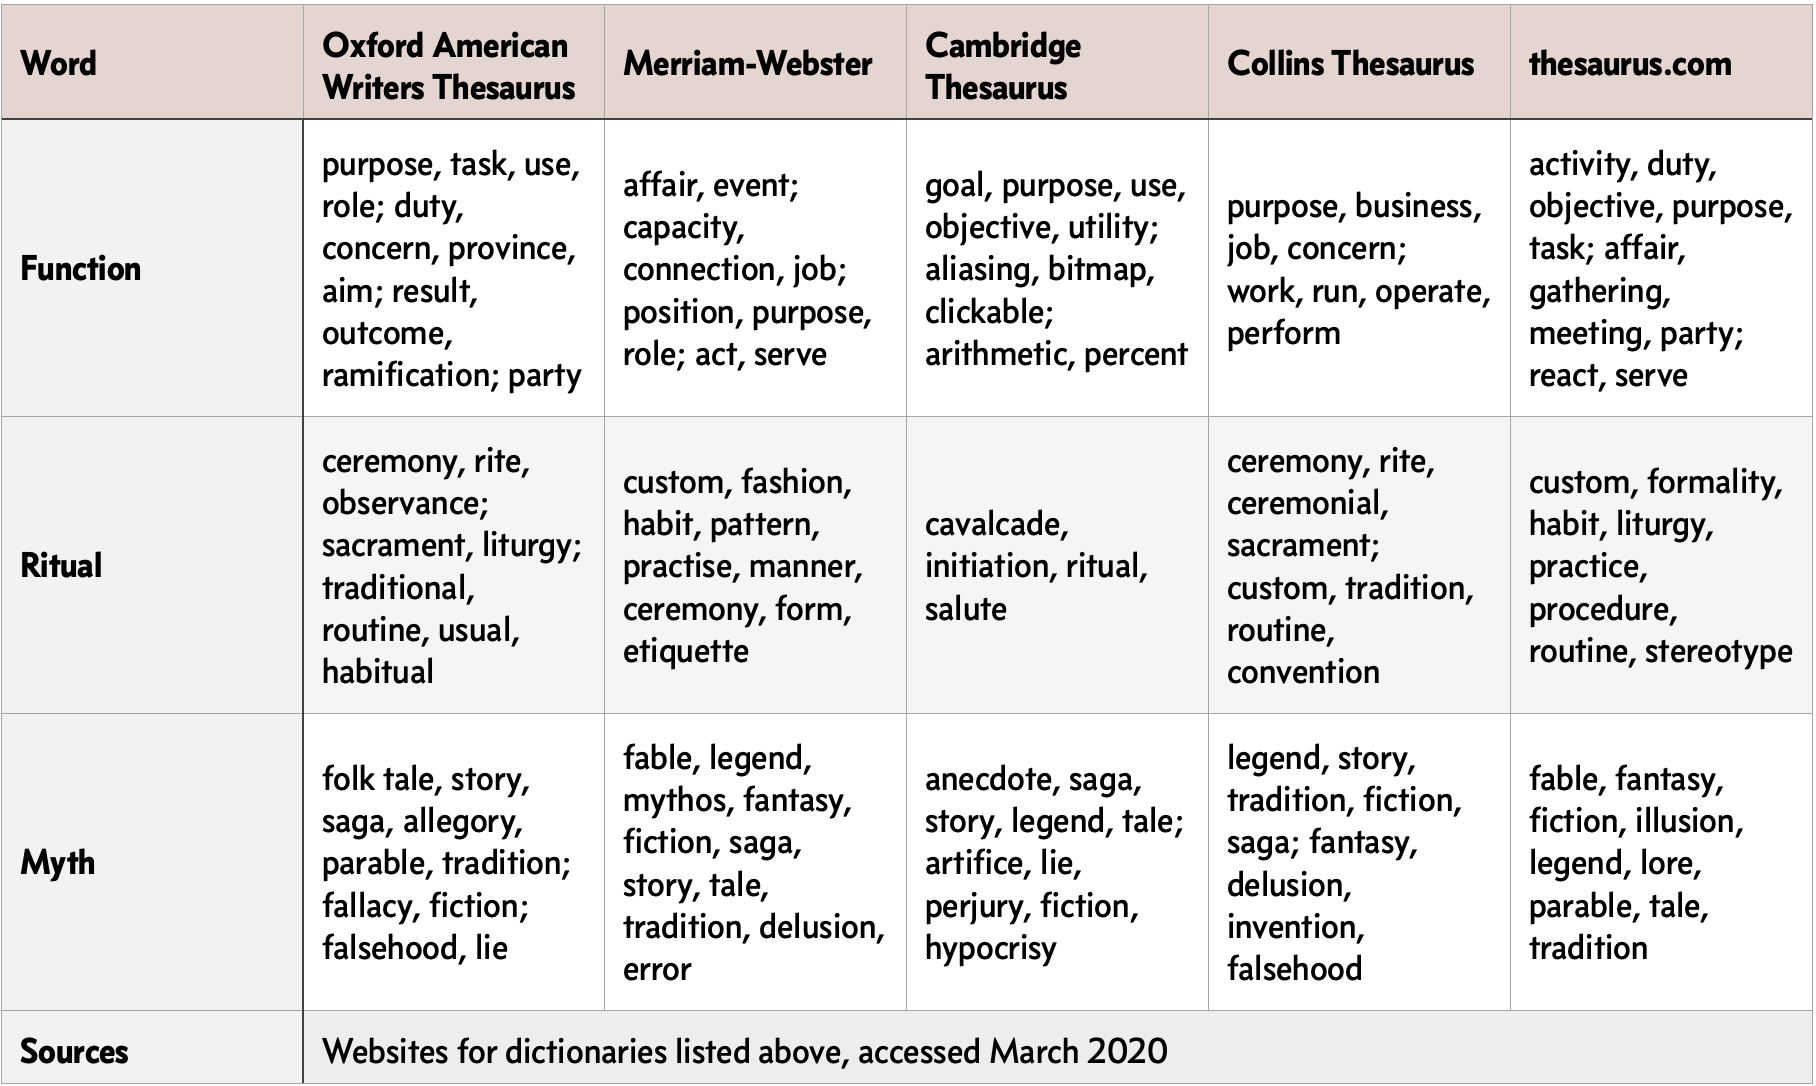
\includegraphics[width=1.19\linewidth]{table1.png}
  \caption{Related Words list --- a summarised range of results from selected dictionaries. the full table is available on our research website \href{https://meaning.pub.}{meaning.pub}.}
  \label{tab:table1}
\end{figure}
\vspace*{1.2em}

In Table 1 we can identify some differences between dictionaries, but largely these volumes have similar patterns.
What can be concluded is that the vocabulary in these dictionaries is formal.
Most dictionaries include informal variants of a word, but usually only one at the end of a long list of more formal terms.

Compiling the complete table of definitions and related words was a tedious and poorly scaleable process.
It is simple not efficient to manually read one dictionary at a time and write down the definitions and synonyms of a word.
The problem is also that the dictionary is becoming a rare book in the home and people will rather go to Google for their questions.
The dictionary is the wrong kind of reference if we want to establish today’s language.
If we want to build a real understanding of natural language used by non-experts, we need to extract the descriptors people use from a different, more casual corpus.

%===================================

\chapter{Corpus Search}

In Figure \ref{tab:table2} we compare different corpora used by computer scientists and linguists for extraction of natural language.
These corpora feature samples from written and spoken English (and other languages), and in some cases are already trained or annotated with vectors to be understood by machine learning programs.

\vspace*{1.2em}
\begin{figure}[!htbp]
  \hspace*{-3.666em}
  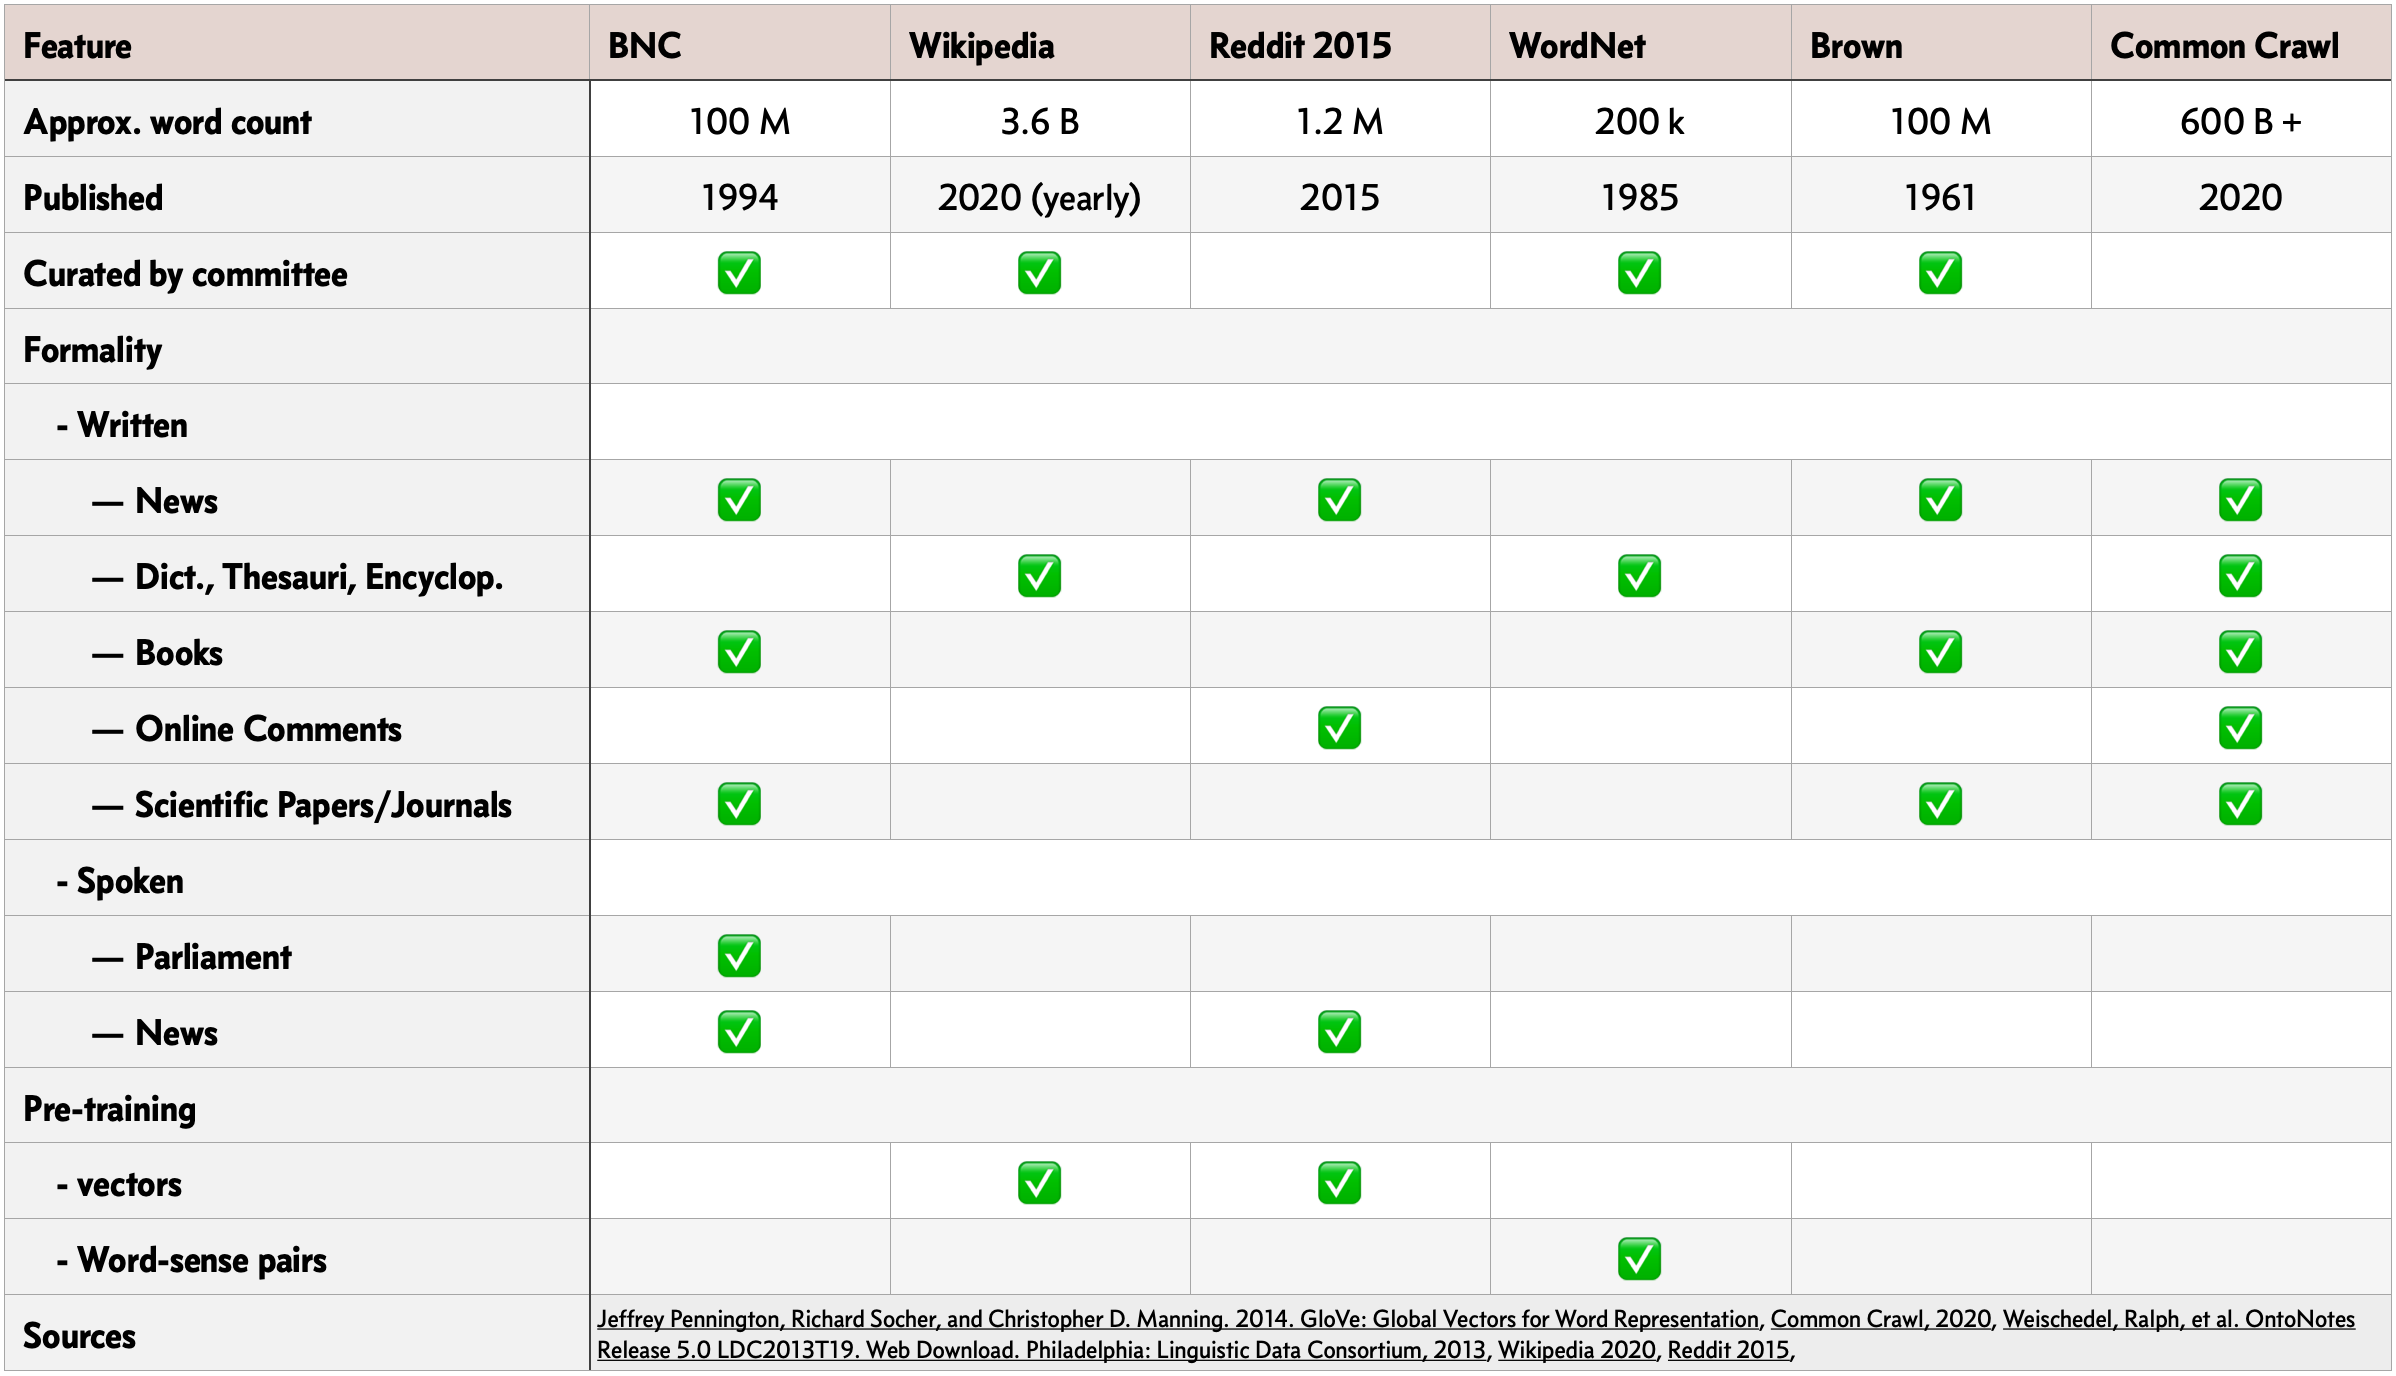
\includegraphics[width=1.19\linewidth]{table2.png}
  \caption{Comparison of selected corpora}
  \label{tab:table2}
\end{figure}
\vspace*{1.2em}

Some of these corpora are on the formal side of the spectrum, similar to our dictionaries.
The contents of these corpora are curated by a committee and contain peer-reviewed journal articles.
On the other side of the spectrum, we have informal corpora such as Reddit or Common Crawl.
These merely scrape an entire website (or in the case of Common Crawl the entire web) and collect all content.
This includes misspellings, made-up words, neologisms, derogatory speech, slang, acronyms and more.
While this may seem undesirable at first, the lack of a committee to filter content can also provide us with the most precise picture of naturally-used language by people.
Our desired corpus should feature a mixture of formal and informal samples, with a focus on the more casual, as we already have the dictionary data for a formal, recognised dataset to compare results against.
Using the right corpus, we can build a semantic network of related terms and explore the relationship of different words with our three focus words.
To build this network we will look at natural language processing, which combines machine learning and linguistics to give a computer the ability to process, analyse and understand language.
The different types of machine learning algorithms are defined by their context of use, their approach to problem solving and the data they process.
The defining factor for the quality of the output is the quality of the input.
We need to select
a good corpus. This corpus should be versatile enough to include the context we want, but also know about other contexts so that our model can learn what to ignore.
It will at first be used to train our model with a given algorithm and later we can plug our trained model into a new corpus to see how well it detects our desired words and if it can find new previously undiscovered terms.

%===================================

\chapter{Phase 1: Natural Language Processing (NLP)}

NLP focuses on expressing language in a way that is intelligible to machines.
It combines the power of linguistics and computer science to study the rules and structures of language, and create intelligent systems capable of understanding, analysing, and extracting meaning from text and speech (MonkeyLearn, 2019)\cite{monkeylearn2019}.

The field dates back to Alan Turing and his eponymous benchmarking test (1950)\cite{turing1950}.
Early applications were in translation work (IBM, 1954, ALPAC, 1966)\cite{hutchins2004}\cite{committee1966language}, rudimentary psycho-analytical chat bots (Weizenbaum, 1966)\cite{weizenbaum1966} and conceptual ontologies or knowledge graphs (Powers, 1984)\cite{powers1984}.

With the advent of machine learning in the 1980s, there was a revolution in the training of NLP models --- away from hand-curated rules, to an approach based more on probability and “learning by doing”. Machine learning algorithms learn automatically through experience (Mitchell, 1997) \cite{mitchell1997} and build a model based on a dataset.
Using this model, the algorithm can recognise statistical patterns and make predictions.

With part-of-speech tagging (POS tagging is the process of identifying words as nouns, verbs, adverbs, etc.) and the introduction of large text corpora (Brown, 1961, WordNet 1985) \cite{brown1979} \cite{wordnet1995} it became possible to build functioning machine translation models.
The next evolution came with word embeddings.
The next sections give a brief overview of the current standards in NLP.

%===================================

\section{Word Embeddings}

Corpus-based semantic representations (word embeddings) use statistical patterns in the text to map words in a vector space (Altszyler et al., 2017) \cite{altszyler2017}.
In the semantic word-space, terms with a similar meaning tend to form a cluster.
This relies on the concept that words with similar meaning appear in similar contexts (Harris, 1954) \cite{harris1954}.

Depending on the algorithm used to calculate the embeddings, different features (Figure \ref{tab:table3}) are used.
This is where the field becomes too opaque for us to offer a precise explanation, so we focused on what we can explain.

[Figure \ref{tab:table3} on next page]

\vspace*{1.2em}
\begin{figure}[!htbp]
  \hspace*{-3.666em}
  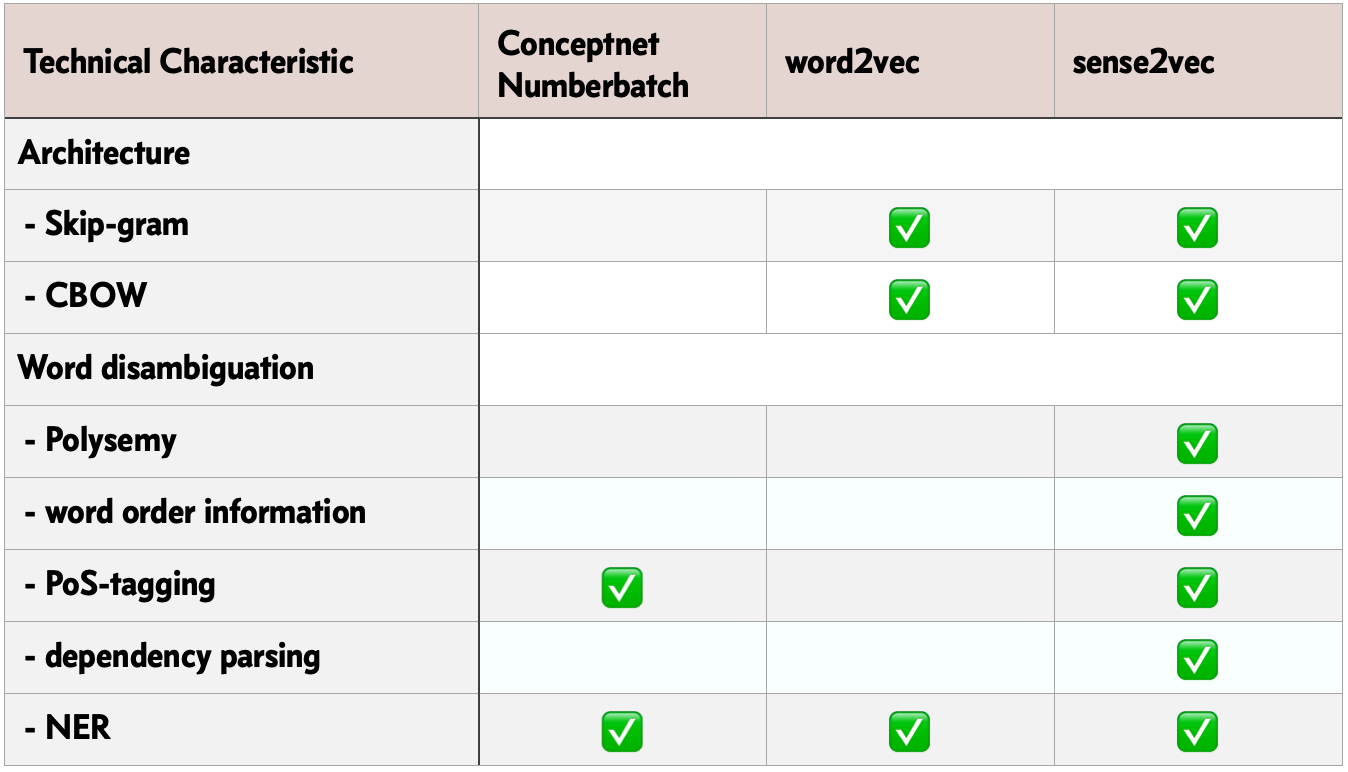
\includegraphics[width=1.19\linewidth]{table3.png}
  \caption{comparison of selected algorithms}
  \label{tab:table3}
\end{figure}
\vspace*{1.2em}

Named-entity resolution, or NER, parses a collection of words that belong together as one, for example New York City, or Pablo Picasso.
This entity is assigned a vector, rather than its individual parts.

Polysemy is the disambiguation of words with multiple meanings.
This has to do with POS, but is more nuanced since it looks at the context in which a word is used.
Two words can have the same spelling, same POS but different meanings.
Function is a good example.
Are we talking about a social gathering, the role at a company or the operation of a device? Here, each meaning, or sense, is assigned a unique vector.

Dependency parsing is the representation of words’ relation on each other, recognising the syntax of a sentence and learning about subject, object and action.

The two main architectures for word embeddings are CBOW (Continuous Bag-of-Words) and Skip-Gram.
In the CBOW architecture the goal is to output a focus word from a number of surrounding context words.
In the Skip-Gram architecture, our input is the focus word and we want to maximise the probability of outputting the context words.

%===================================

\section{word2vec}

Word2vec (Mikolov et al., 2013) \cite{mikolov2013} is used to produce word embeddings.
It takes words from a corpus and produces a vector-space with hundreds of dimensions, each word having their unique vector.
Words that are related by context in the corpus are located closely in the word-vector-space.

To get better results, Mikolov et al. describe a subsampling method to counter the imbalance in a data set between frequent words (“to”, “and”) that are not telling us anything unique about our input, and rare words which are more valuable in guiding the model.

In the Skip-Gram model, each word is defined based on the characters that compose it (its spelling) and is assigned a vector, a direction of meaning, capturing their semantic and syntactic information (Maas \& Ng, 2010) \cite{maas2010}.
That means that function, ritual and myth are assigned an individual vector, but also functions, functional and functionality, because these words are all spelled differently.
In word2vec, polysemous words share a same vector.

%===================================

\section{sense2vec}

The work by Reisinger \& Mooney (2010) \cite{reisinger2010} takes a new approach on vector-space word-sense disambiguation by first clustering the contexts in which a word appears to then encode multiple meanings, or senses, for polysemous words.
The methods of Chen et al.\ (2015) \cite{chen2015} or Rothe and Schütze (2015) \cite{rothe2015} use Princeton’s WordNet to find the number of definitions a word has instead of looking at a preset number of clusters.
These additional steps improve the quality of the output, but at the cost of heavier computation (Trask, 2015) \cite{trask2015}.

Sense2vec uses POS-tagging (Horn, 2017) \cite{horn2017} as well as named-entity resolution (NER) to assign each meaning of a word their own lexical unit.

%===================================

\section{NLP Libraries}

A library (or tool) combines the features of one or more algorithms and lets us plug in corpora to do our training and data analysis on.

\vspace*{1.2em}
\begin{figure}[!htbp]
  \hspace*{-3.666em}
  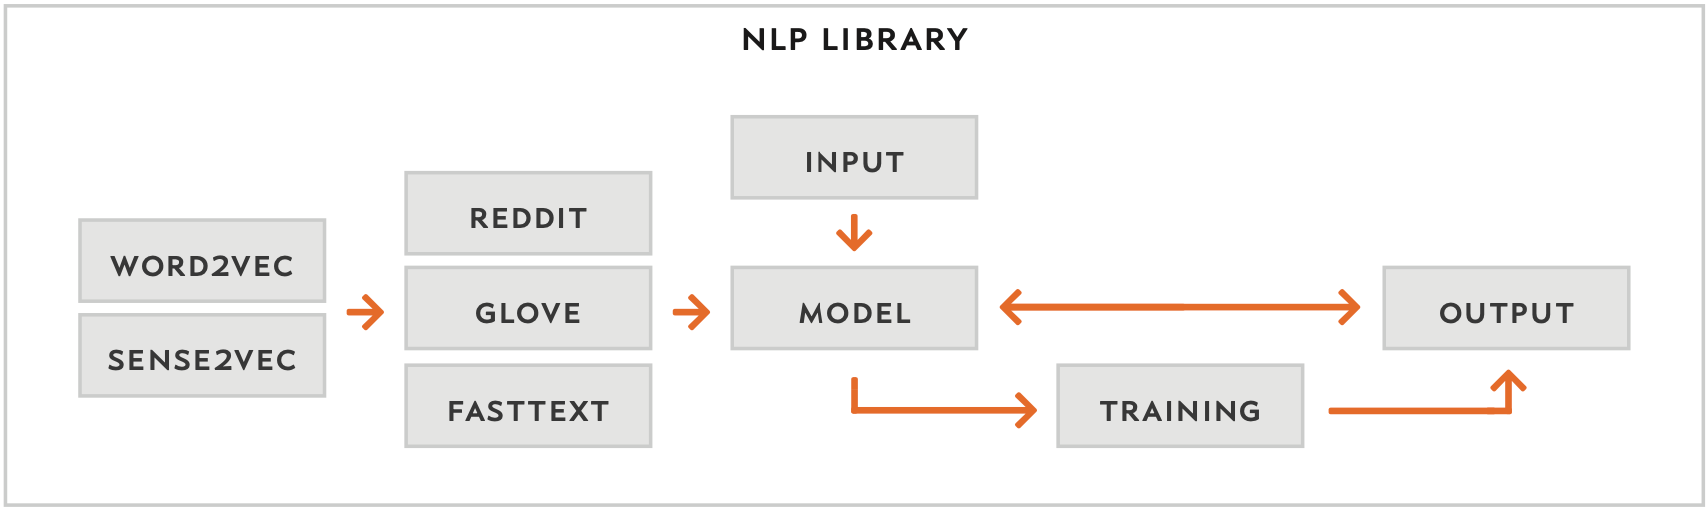
\includegraphics[width=1.19\linewidth]{fig1.png}
  \caption{Flowchart of library's function}
  \label{fig:figure1}
\end{figure}
\vspace*{1.2em}

Figure 1 outlines the function of a library.
It uses a word embedding algorithm to preprocess a corpus to be fed into a model.
This corpus can be vectorised or raw text.
An input word or document can be added to the model as a seed.
This can be enough to provide an output.
However, the result may not be in the desired word-vector space (context) and further training may be required.
The back-and-forth between model training and output evaluation may have to be repeated for a dozen instances before desired results are visible.

NLTK is one of the most-recommended libraries, however it is quite large and not obvious to the beginner.
For us, it is crucial that we use a production-ready library, as we cannot invest the time to learn multiple tools.
If one library provides good documentation in the form of tutorials and can be used on its own, it becomes a viable candidate for our selection.
We also established that we need sense2vec in our algorithms as it will theoretically provide more intelligent results.
The sense2vec architecture also offers polysemous word-sense disambiguation, which is crucial to differentiate between the different meanings of function.

Lemmatisation can reduce derivations of a same word (word, words, wording) to its stem, or lemma.
All possible derivations of a word’s lemma make up the lexeme of this word.
Stemming is similar, but also takes into account conjugation or pluralisation where the spelling or a word changes completely.

We want the library to have a simple way of training.
Since the words we are using can exist in many contexts, we will want to guide the model in the right direction.
This can be done by evaluating the output and repeating the process with trained data.
We are currently seeing this stage as a potential source of poor results.

Other basic features of libraries include tokenisation, where each word and symbol in a sentence is identified as its own token, and classification, where words or named entities can be categorised into a common group like sports or economics.

\vspace*{1.2em}
\begin{figure}[!htbp]
  \hspace*{-3.666em}
  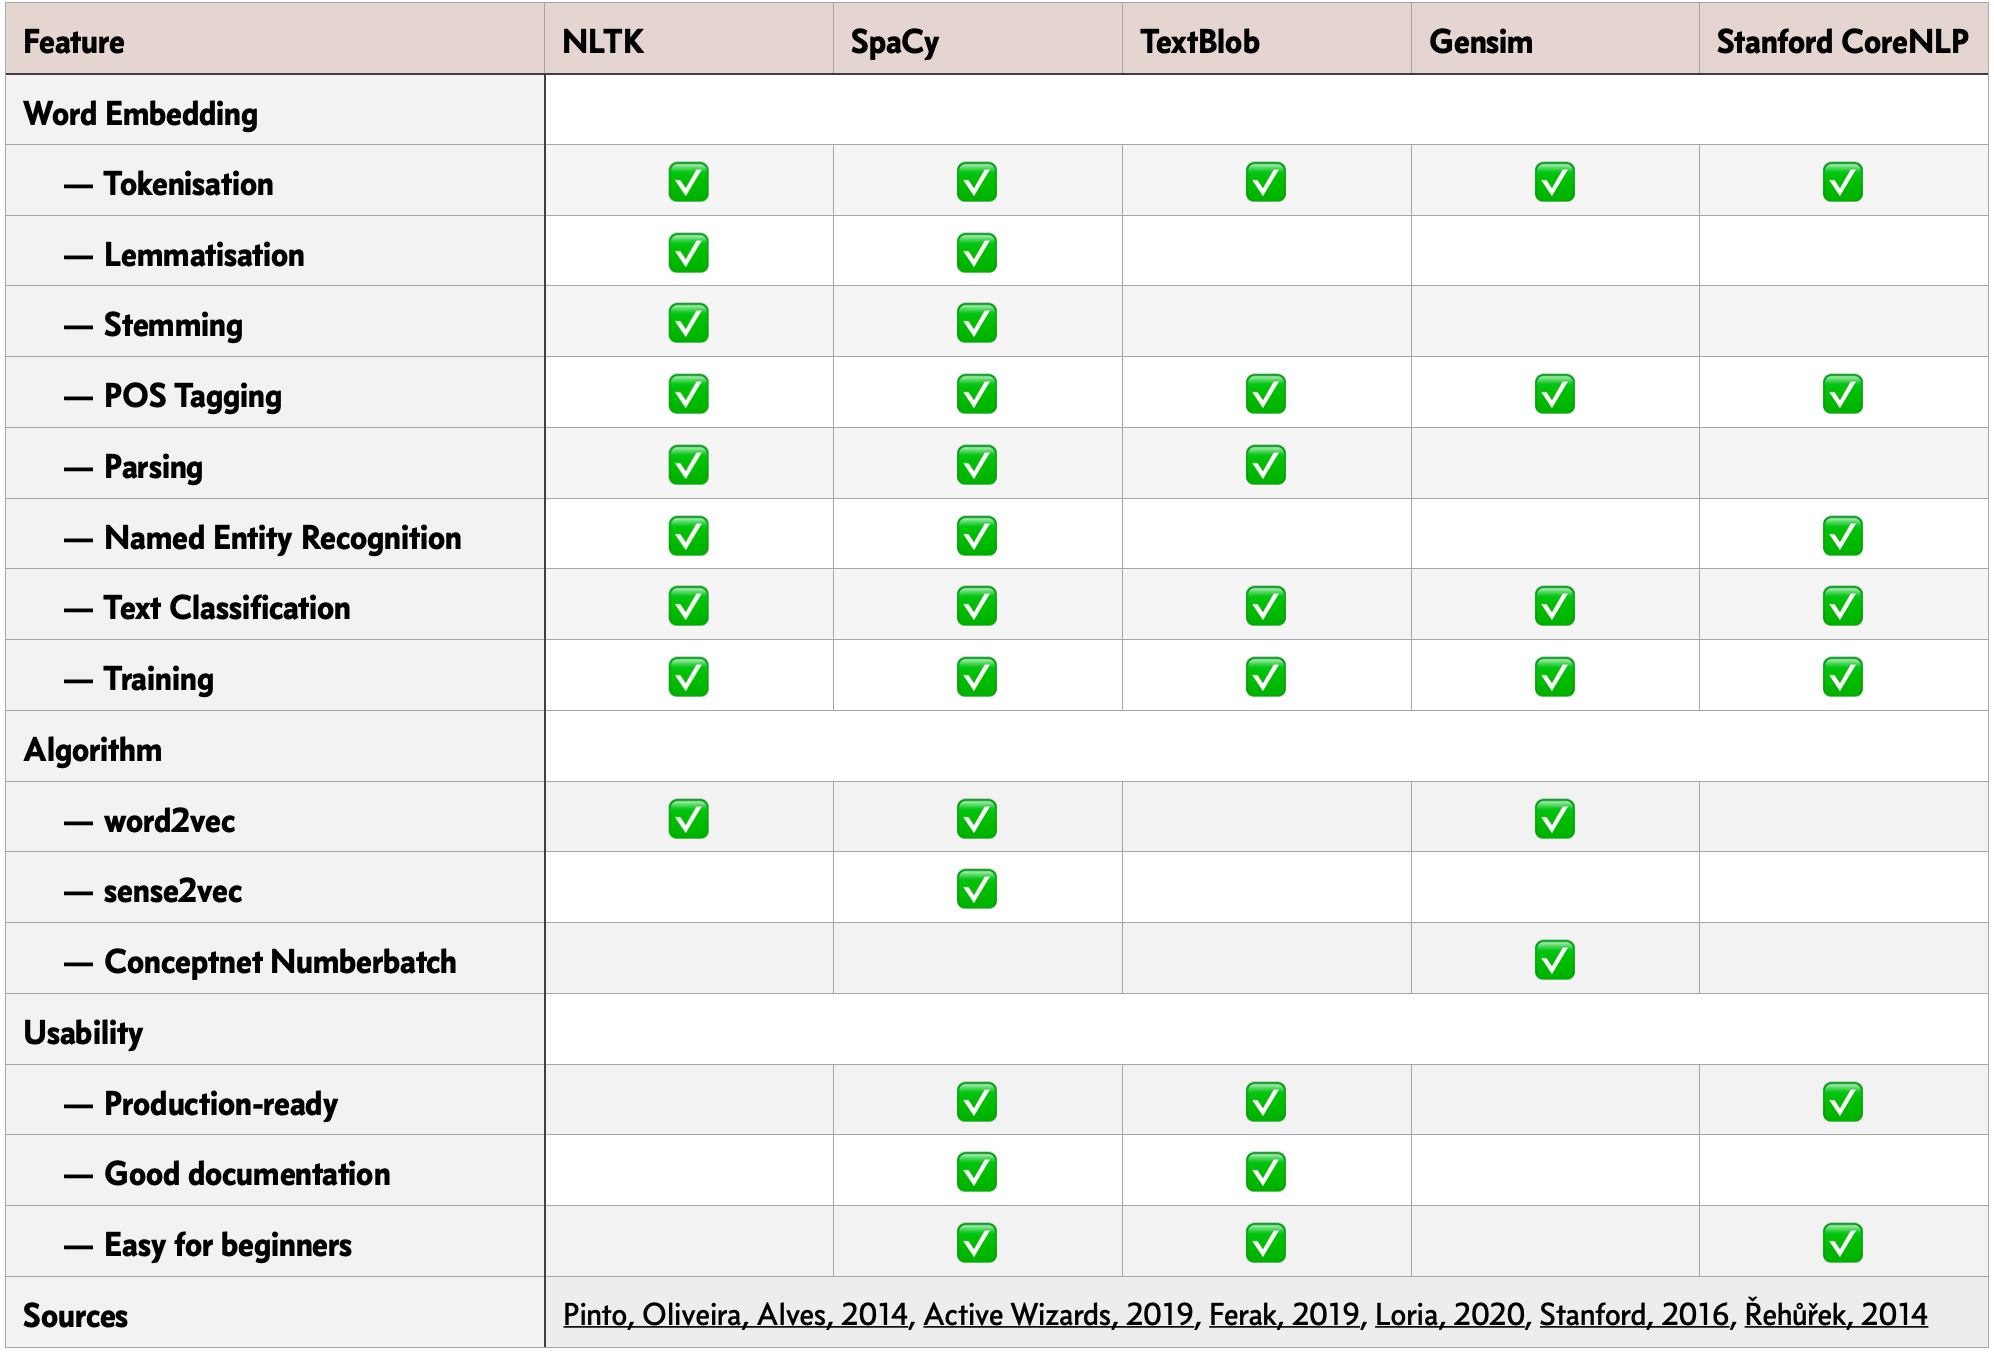
\includegraphics[width=1.19\linewidth]{table4.png}
  \caption{comparison of selected NLP libraries}
  \label{tab:table4}
\end{figure}
\vspace*{1.2em}

From Figure \ref{tab:table4} above, SpaCy can be identified as the most promising candidate.
It has most of the features and although it’s relatively new and not as established as NLTK, it has a comprehensive documentation along with tutorials that we can follow along to learn the tool.
From our research, it seems like a favourite among new NLP projects for its speed and ease of use.
The makers of SpaCy, \href{https://explosion.ai}{Explosion}, also have a text classification and training tool called Prodigy that can be used for text classification.
Text classification can help us identify senses of our focus words in a corpus.

In theory, once the model is sufficiently trained we can test results from different corpora and find related words based on context, from formal to informal.
So far, however, no results have been achieved that could beat those provided by online demos where we had no control over training the model to focus on our desired word-vector space.

We reached out to Explosion and they provided us with a free research license of Prodigy, a tool that would normally cost \$400.
We are currently still evaluating and learning Prodigy.
Once we produced results aligning with our goal, we will purchase the tool as to not appear biased towards the developers.

%===================================

\chapter{Results from NLP}
\section{Technique for online tools}

In parallel to comparing and selecting a good library for us to use we looked into ready-to-use tools to build semantic networks.
Since approached to NLP are problem-specific, there are no comprehensive programs with a user interface where we can select a corpus and receive output based on some input words. 
What we found were examples of application or proofs of concept by companies with tools that are up to the individual to design and program to their exact needs.
Examples such as those by Explosion (SpaCy), Turku University’s NLP Group, Google’s Tensorflow, a demo by Anthony Liu, or Radim Řehůřek (Gensim) have a setting to select vector dimensions or switch from CBOW to Skip-Gram, but mostly a simple input into a textfield will yield results.
Other examples such as ConceptNet or Facebook’s FastText required a small amount of programming in Python or depended on Gensim to function and parse the vectors.

\subsection{ConceptNet}

ConceptNet is a freely-available semantic network to find related words in its ontological multi-lingual database from Open Mind Common Sense, Wikipedia, WordNet, etc and was developed by Speer et al.\ (2018) \cite{speer2018}.
When searching for a word, the results are displayed in classes --- synonyms, related terms, types of, derived terms, ways of, things used for, context of, word forms, etymological relatives, antonyms and more.
The tool understands different levels of dependency, can detect if a word has an effect on another word and what the use of the word is.
Depending on the input word, the quality of these dependencies and related words varies widely.
Figure \ref{fig:figure2} is a screenshot from ConceptNet website, comparing results for x is capable of illustrating the differences when looking up regular words versus rare words.
With decreased frequency of use the models have a hard time understanding the relationships the word has on others.
The results from ConceptNet’s website are output in all languages it can find related words for.
This overcrowds the results.
ConceptNet have a clearly-written API on GitHub with examples of related word queries filtered to English and including or excluding certain parameters.
The given parameters for a word can be viewed in the API.
The complete semantic network for myth can be viewed at \url{api.conceptnet.io/c/en/myth}.
This pattern matches for all word queries.

\vspace*{0.2em}
\begin{figure}[!htbp]
  \hspace*{11em}
  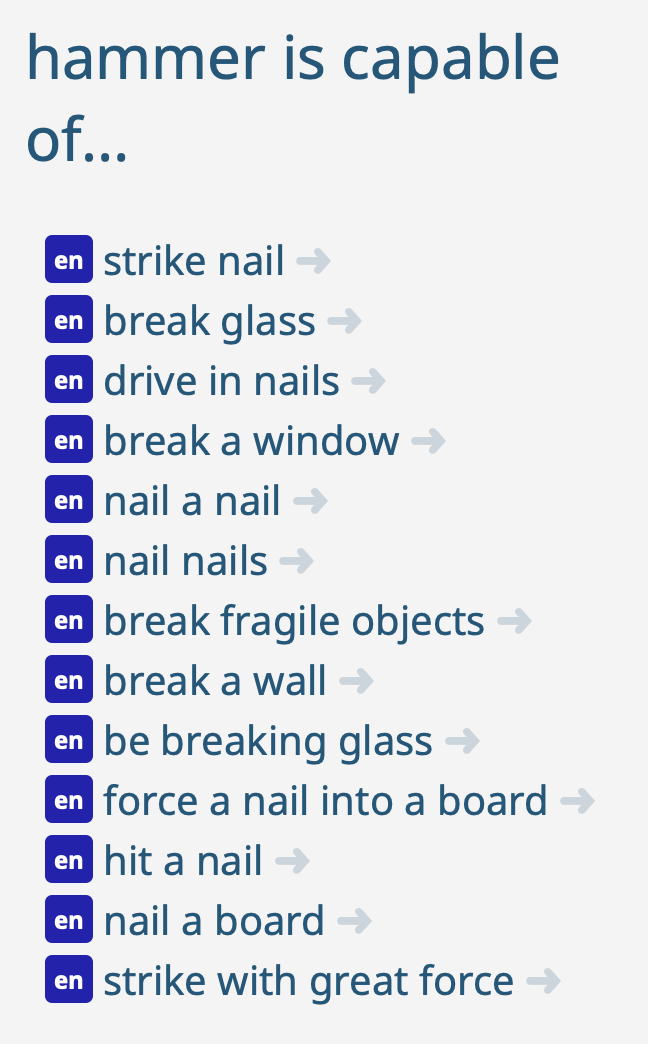
\includegraphics[width=0.4\linewidth]{fig2.png}
  \caption{ConceptNet example results for \emph{Hammer}}
  \label{fig:figure2}
\end{figure}
\vspace*{0.2em}

We wrote a script that gets the related words of our input term, removes the derived terms and forms of the word, and outputs the results in a table.
The API calls in our script are humanly-readable and go as followed:
First, we get the related words using \bverb{http://api.conceptnet.io/related/c/en/alpha}, where alpha is our input word.
Then we call derived terms \bverb{http://api.conceptnet.io/query?node=/c/en/alpha\&rel=/r/DerivedFrom} and forms of \bverb{http://api.conceptnet.io/query?node=/c/en/alpha\&rel=/r/FormOf} and subtract both from the related words list.
The difference is output into a table which we copied into Table \ref{tab:table5}.
We also attached weighting to the related terms, the meaning of the weighting however is not qualifiable, nor is a low weighting an indicator for uninteresting words.
We wrote the script to have flexibility over the number of output words and compared the results with 10, 20 and 50 output words per term.
The results were poor with 10 results and we did not gain further insight looking at 50 results.

\subsection{Turku University’s NLP Group}

Turku University in Finland have an NLP department which maintains an online demo of word2vec trained on 4.5 billion Finnish words from the Finnish Internet Parsebank, a project which they describe with three goals:
First to create a tool with automatic syntactic analyses, second a complete classification database and third an online user interface to interact with, which is their demo in Figure 3.

\vspace*{1.2em}
\begin{figure}[!htbp]
  \hspace*{-3.666em}
  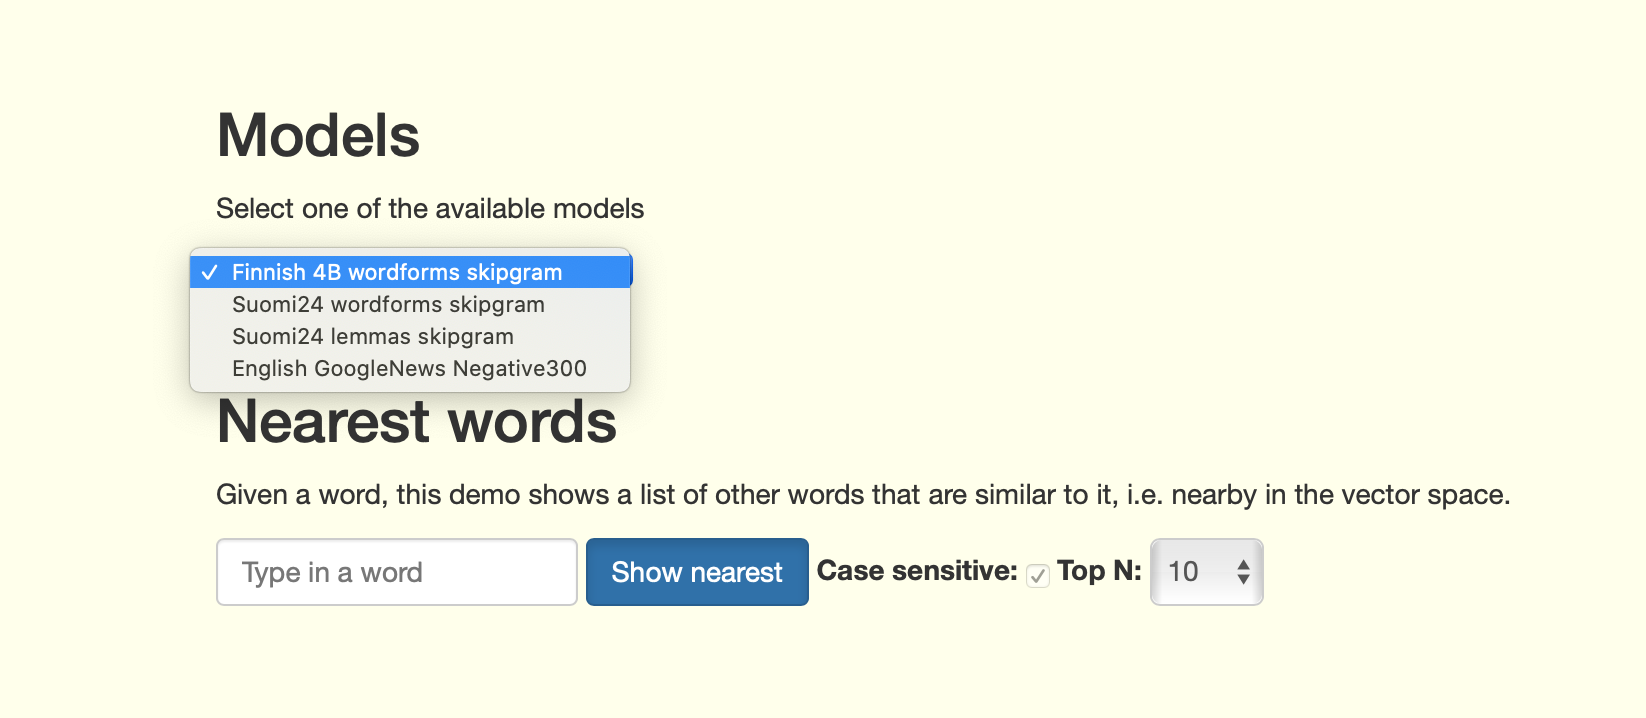
\includegraphics[width=1.19\linewidth]{fig3.png}
  \caption{Turku University’s NLP Demo at \url{http://bionlp-www.utu.fi/wv_demo/}}
  \label{fig:figure3}
\end{figure}
\vspace*{1.2em}

Their demo allows for the selection of different models and next to searching
for nearby words also offers the possibility to view the numeric similarity of two words and to compute a word analogy akin to word2vec's example \bverb{king - man + woman $\approx$ queen} (Mikolov et al., 2013) \cite{mikolov2013}.

We did not use the comparison or analogy features and instead focused on getting 10 related words for a single input word and repeated the process for each of our three focus words.
The results were copied into Figure \ref{tab:table5}).

\subsection{Anthony Liu’s demo}

We found another word2vec demo this time using common English words as a corpus.
It was created by Anthony Liu, an MIT computer scientist with a specific focus on theoretical neuroscience and AI.

\vspace*{1.2em}
\begin{figure}[!htbp]
  \hspace*{-3.666em}
  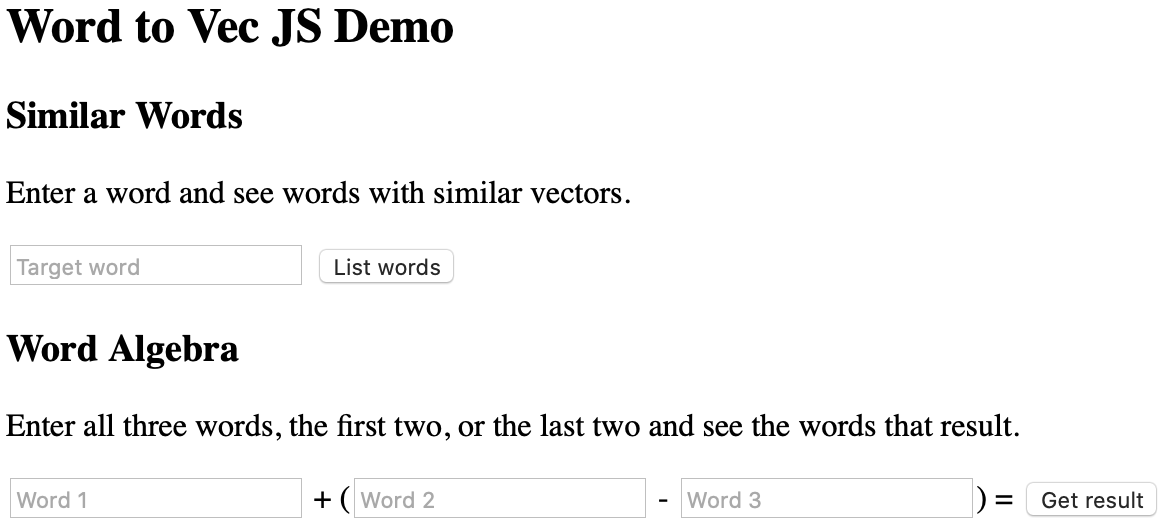
\includegraphics[width=1.19\linewidth]{fig4.png}
  \caption{Word to Vec JS Demo}
  \label{fig:figure4}
\end{figure}
\vspace*{1.2em}

This demo (Figure \ref{fig:figure4}) also has the option for word algebra which we forwent in favour of finding 10 related words.

\subsection{Gensim + FastText, Gensim + GloVe}

FastText by Facebook is a library for text classification.
It includes models with one million vectors trained on Wikipedia and two million on Common Crawl.

To use FastText, we had to include it in a Gensim wrapper as it doesn’t have a ready- to-use online demo.
GloVe is an algorithm by Stanford’s NLP department that also uses vectors trained on Wikipedia and Common Crawl, with 400.000 and 1.900.000 words respectively in its vocabulary.

Gemsim can be installed and ran in a Python script using import gensim.
We then loaded the the pre-trained FastText vectors from Wikipedia and later GloVe into Gensim with the command \bverb{gensim.models.KeyedVectors load\_word2vec\_format(‘vectors.vec’)}.
Then we output the 10 most similar results for our focus words using \bverb{most\_similar(‘word’, topn=10)}.

\subsection{SpaCy + Reddit}

SpaCy’s developers, Explosion, have an online demo (Figure \ref{fig:figure5}) of sense2vec using the social discussion and news website Reddit.
In the demo it is possible to input a word and to specify its part-of-speech as well as which year to pick data from.
This lets people compare the change of meaning a word has over time.
The data available is form 2015 and 2019, so while there are no universal linguistic shifts in such a short period, it can be observed that occurances of the word trump now refer to the American President, when before it was linked to ranking.

\vspace*{1.2em}
\begin{figure}[!htbp]
  \hspace*{-3.666em}
  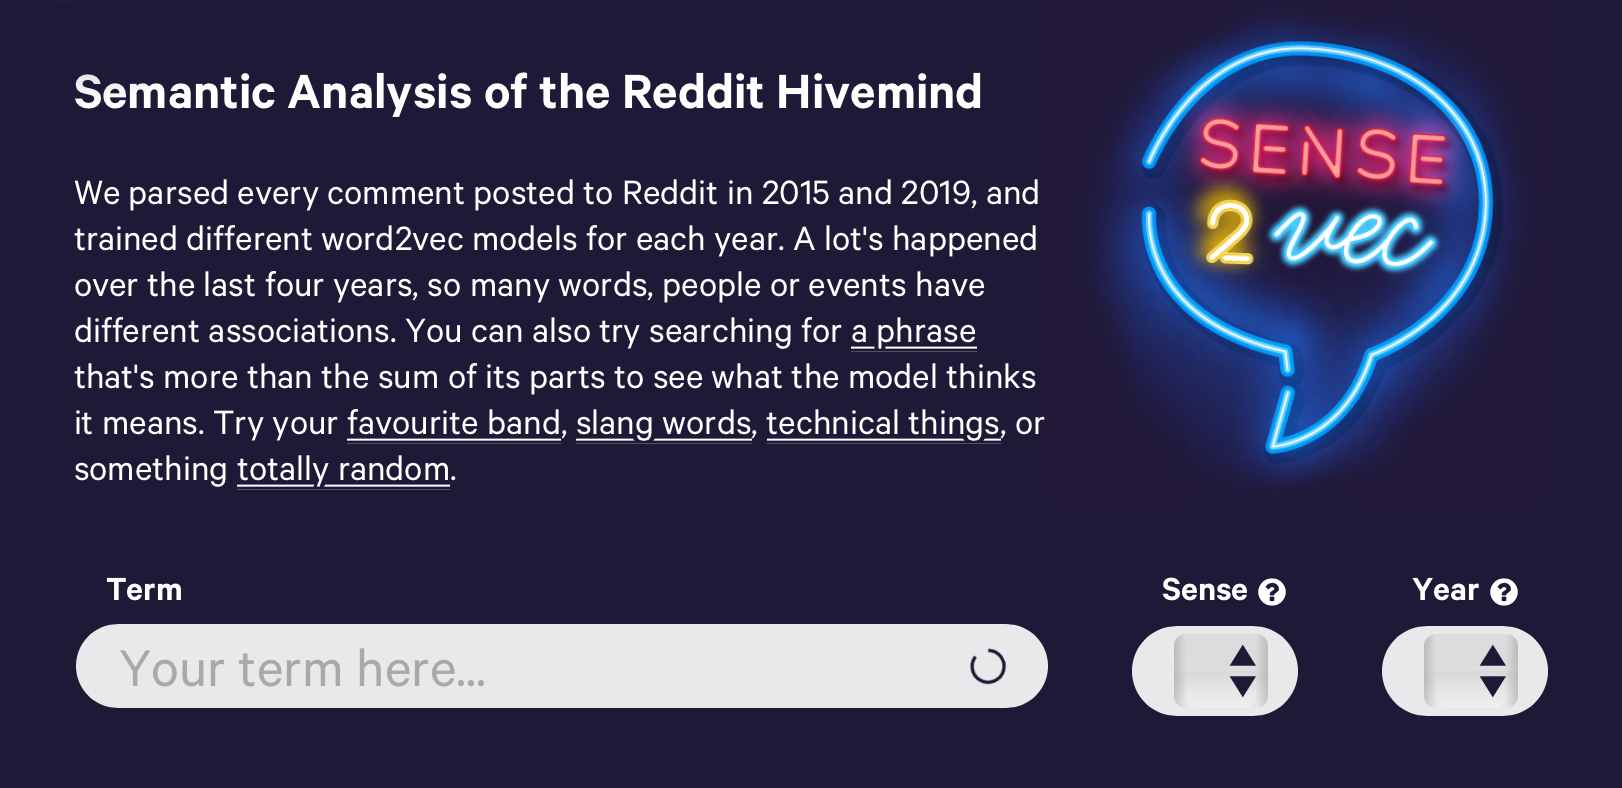
\includegraphics[width=1.19\linewidth]{fig5.png}
  \caption{sense2vec Demo}
  \label{fig:figure5}
\end{figure}
\vspace*{1.2em}

\subsection{Tensorflow Project}

The TensorFlow Embedding Projector by Google is an open-source tool for interactive 3D visualisation and interpretation of embeddings (Smilkov et al., 2016) \cite{smilkov2016}.
It is used to graphically represent high-dimensional embeddings and lets us visualise the relationship of words in our vector-space (Figure \ref{fig:figure7} on the next page).
The online demo we are working with uses a corpus of 25.000 movie reviews from IMBD, the internet movie database.
These movie reviews contain a wide variety of words without being too informal or technical.

We won’t get into details about their data visualisation attributes in this paper, more background information can be found in the paper published by Distill, a peer-reviewed scholarly online journal dedicated to machine learning research, “How to Use t-SNE Effectively” by Wattenberg et al. (2016) \cite{wattenberg2016}.

To read data, we searched for our focus words, increased the points to 1000 and switched to using t-SNE with the standard settings of 200 dimensions, a perplexity of 8, a learning rate of 10 and no supervision.
We let the calculations run for 8000 iterations.
From the table on the right in Figure \ref{fig:figure6}, we copied the 10 first results of nearest points into our results table (Table \ref{tab:table5}).

\vspace*{1.2em}
\begin{figure}[!htbp]
  \hspace*{-3.666em}
  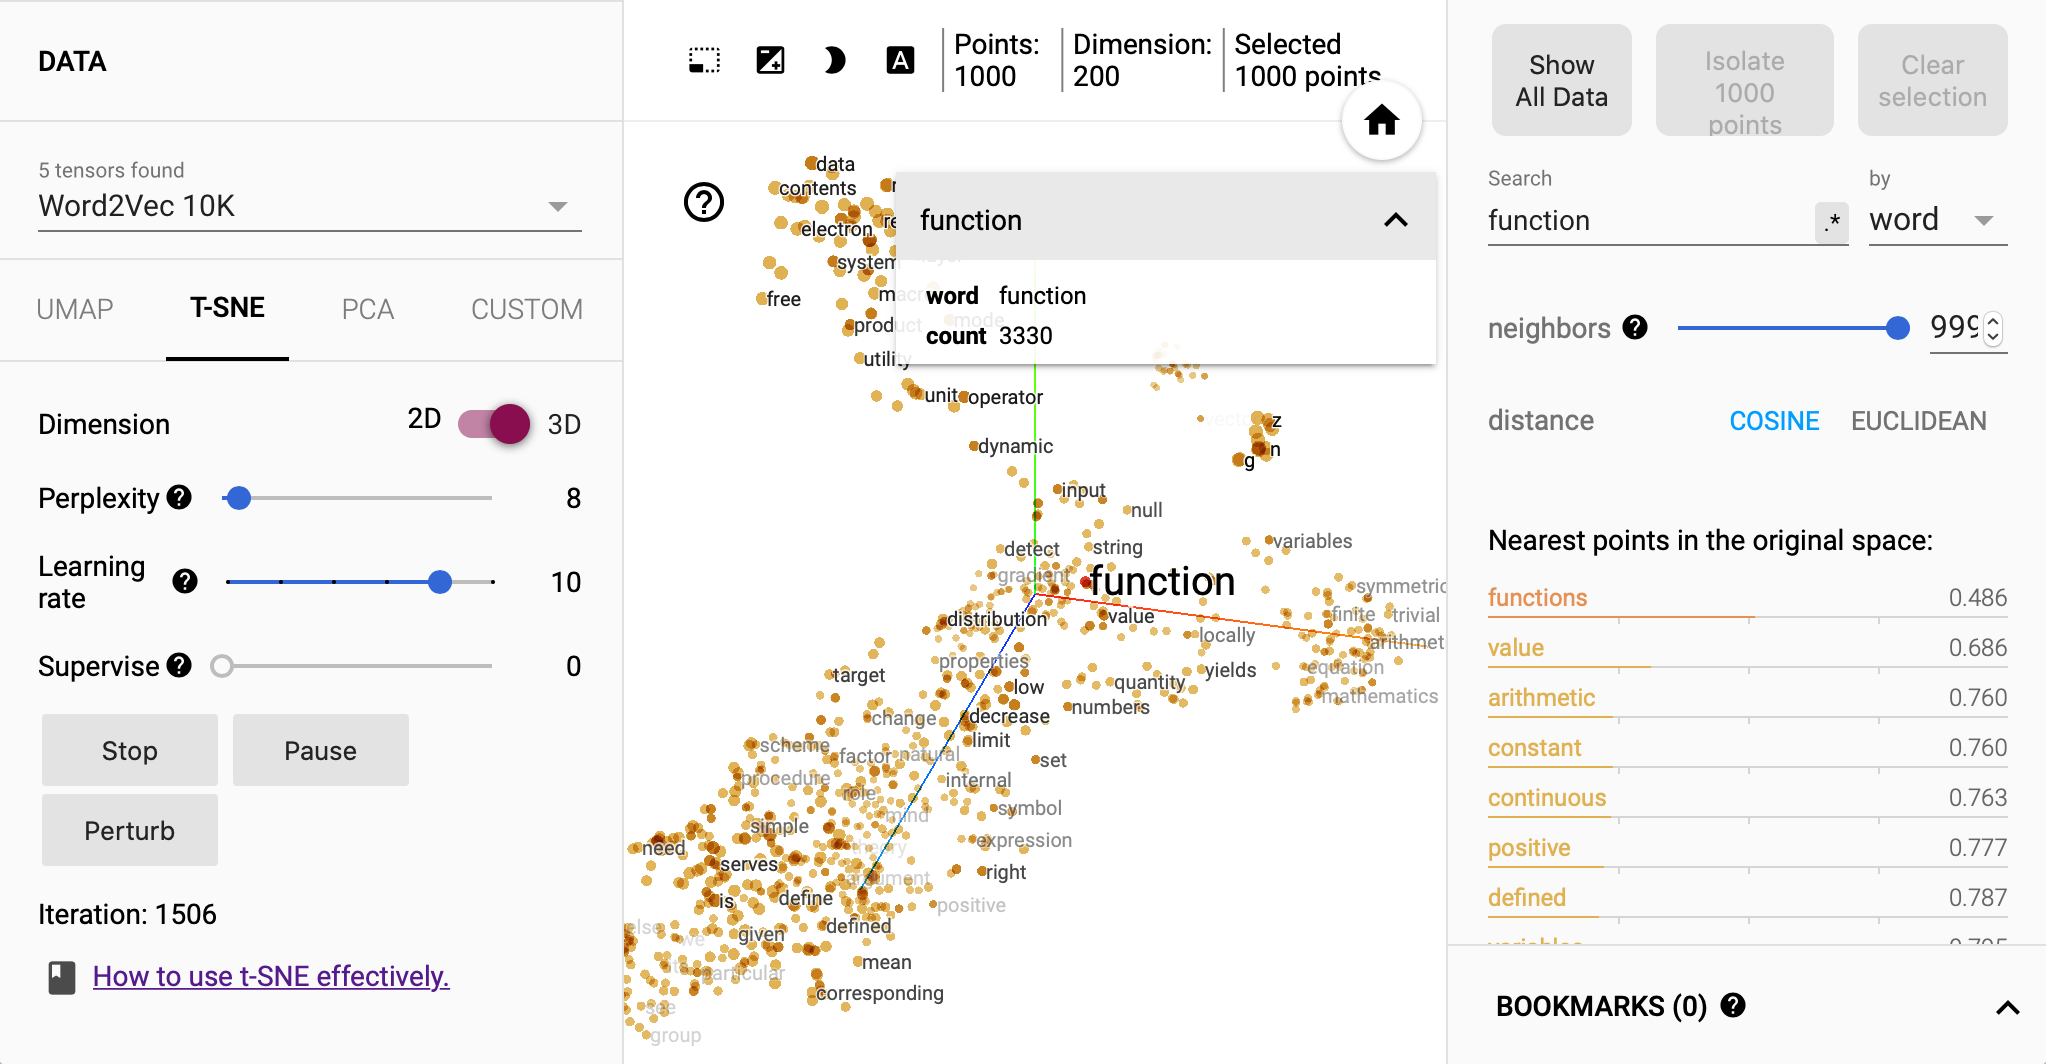
\includegraphics[width=1.19\linewidth]{fig6.png}
  \caption{Tensorflow Projector}
  \label{fig:figure6}
\end{figure}
\vspace*{1.2em}

From Figure \ref{fig:figure7}, \ref{fig:figure8} and \ref{fig:figure9} we can identify word clusters for our three focus words.
While some of these clusters are physically separated from the rest of the words for function and ritual, for myth there are no directly-visible outliers.

\vspace*{1.2em}
\begin{figure}[!htbp]
  \hspace*{-3.666em}
  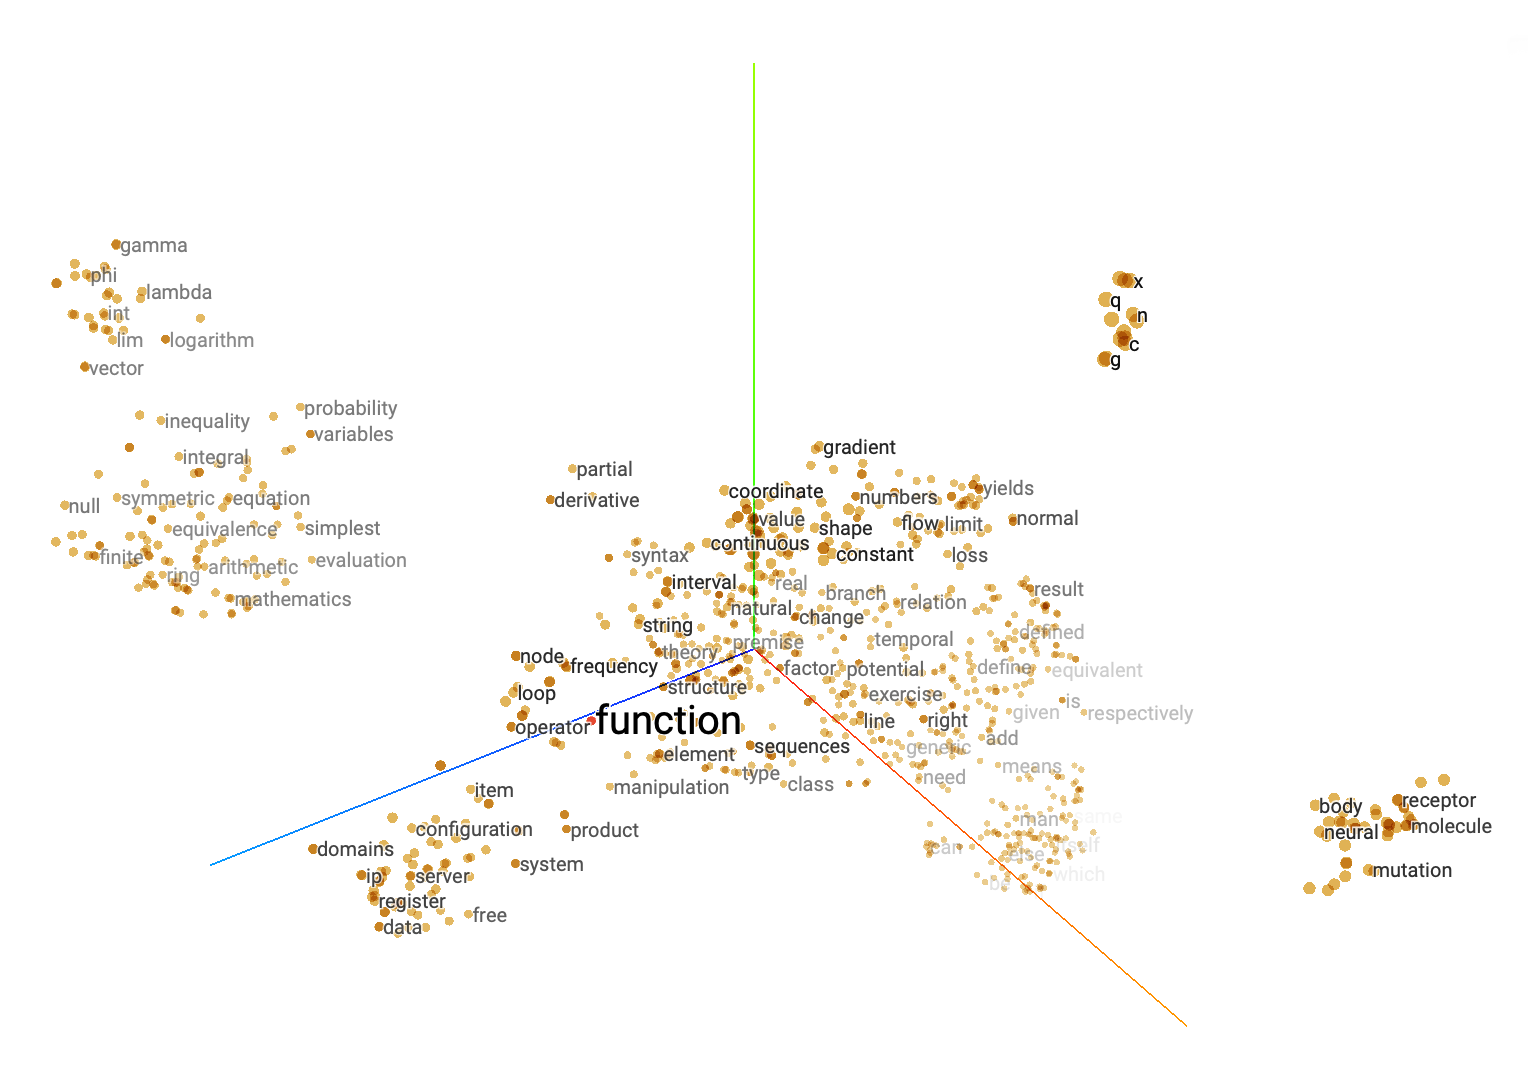
\includegraphics[width=1.19\linewidth]{fig7.png}
  \caption{Tensorflow Projector: Function}
  \label{fig:figure7}
\end{figure}
\vspace*{1.2em}

\vspace*{1.2em}
\begin{figure}[!htbp]
  \hspace*{-3.666em}
  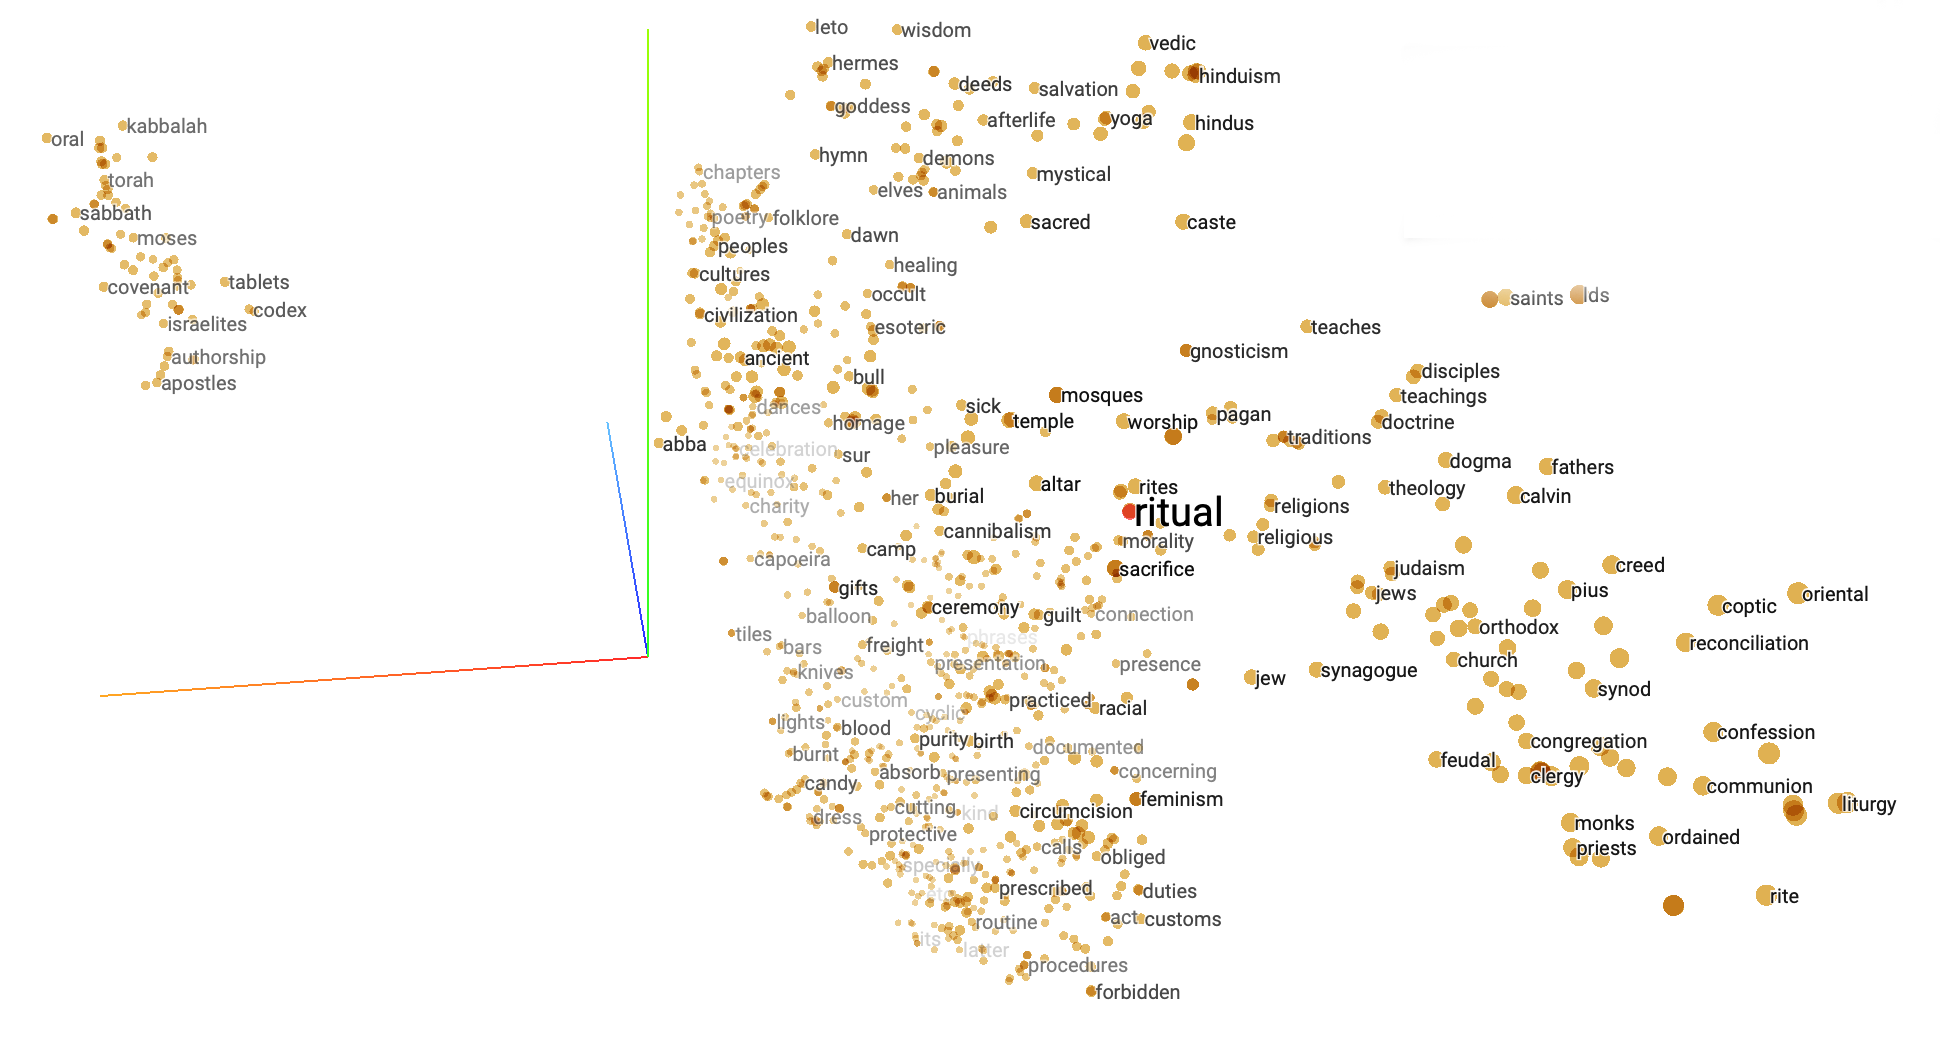
\includegraphics[width=1.19\linewidth]{fig8.png}
  \caption{Tensorflow Projector: Ritual}
  \label{fig:figure8}
\end{figure}
\vspace*{1.2em}

\vspace*{1.2em}
\begin{figure}[!htbp]
  \hspace*{-3.666em}
  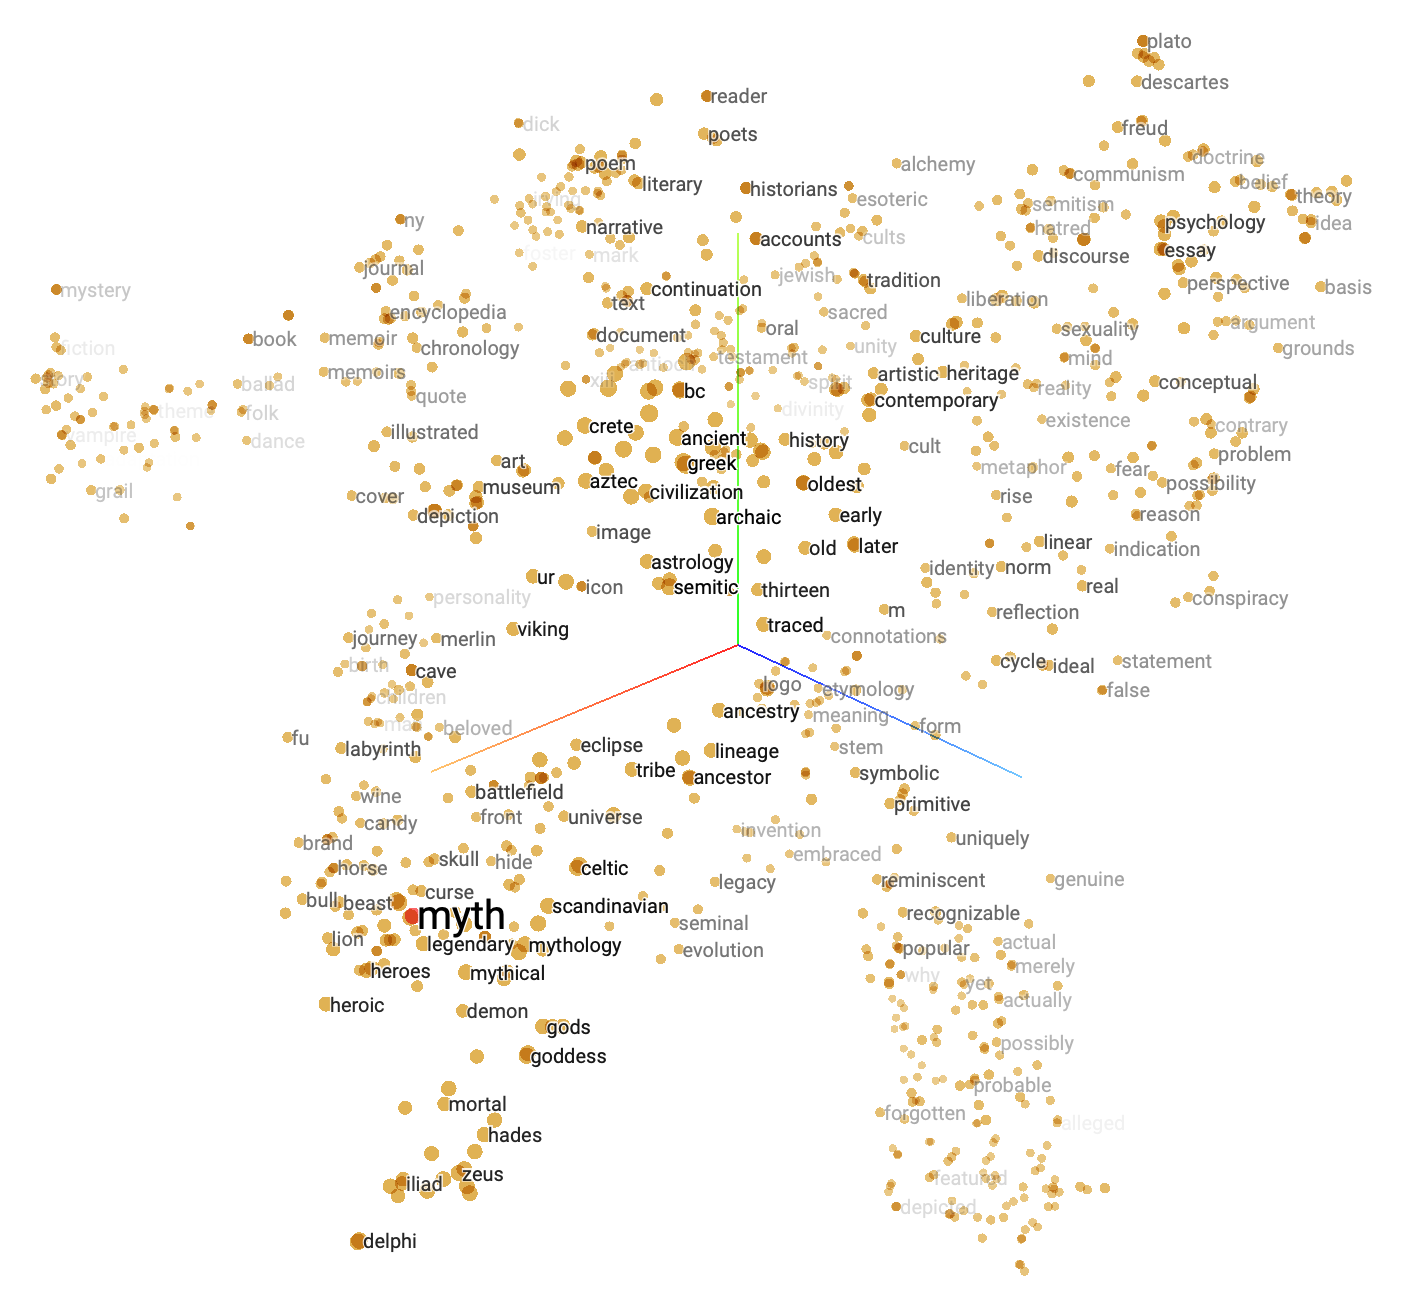
\includegraphics[width=1.19\linewidth]{fig9.png}
  \caption{Tensorflow Projector: Myth}
  \label{fig:figure9}
\end{figure}
\vspace*{1.2em}

\subsection{Polyglot}

Polyglot is another multi-lingual NLP library developed by Al-Rfou et al. (2013) \cite{alrfou2013} with an online demo available on Al-Rfou’s website.
It is not clear from our research if Polyglot is using word2vec for their word embeddings but since the results in Table \ref{tab:table5} vary from other word2vec models, we can assume Polyglot uses more intelligent word-sense disambiguation and handles polysemy as well as stemming and lemmatisation.

\vspace*{1.2em}
\begin{figure}[!htbp]
  \hspace*{-3.666em}
  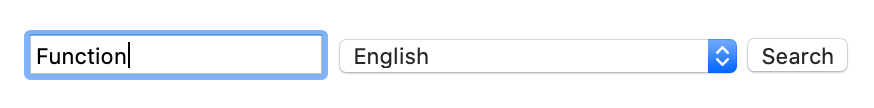
\includegraphics[width=1.19\linewidth]{fig10.png}
  \caption{Polyglot Demo}
  \label{fig:figure10}
\end{figure}
\vspace*{1.2em}

The demo does not have any visible settings (Figure \ref{fig:figure10}) except for language, where it loads vectors from the respective Wikipedia.

%===================================

\section{Technique for SpaCy}

SpaCy’s stand-alone training tool Prodigy was the focus of our NLP research as it checked all boxes in our library comparison and its features addressed everything we understood as being important.
The tool allows us to create a new word category and train a model to recognise words that belong in that category.
To use the word2vec and sense2vec models from SpaCy, we first had to install their tools into a virtual python environment, the details of which process can be read in our blog post about debugging the Prodigy installation.

Once we were set up, we could use the command \bverb{prodigy terms.teach function\_pattern en\_core\_web\_lg --seeds function.txt} to load the \bverb{terms.teach} recipe using the \bverb{en\_core\_web\_lg} model which contains OntoNotes5 and GloVe with 685.000 vectors and 300 dimensions.
The model was loaded with three seed terms (function, task, use) in our function.txt text file.
Prodigy launches a local web-server (Figure \ref{fig:figure11}) where we can graphically see the words to categorise and can accept, reject or ignore words.
We can also undo our classification and revisit a word.

For our results table (Table \ref{tab:table5}) we wrote down the first 10 words that we received from Prodigy without accepting or rejecting them.
This process was repeated for function, ritual and myth using a fresh pattern file for each, where training data is saved to and can be loaded from in a second round of text classification.

\vspace*{1.2em}
\begin{figure}[!htbp]
  \hspace*{-3.666em}
  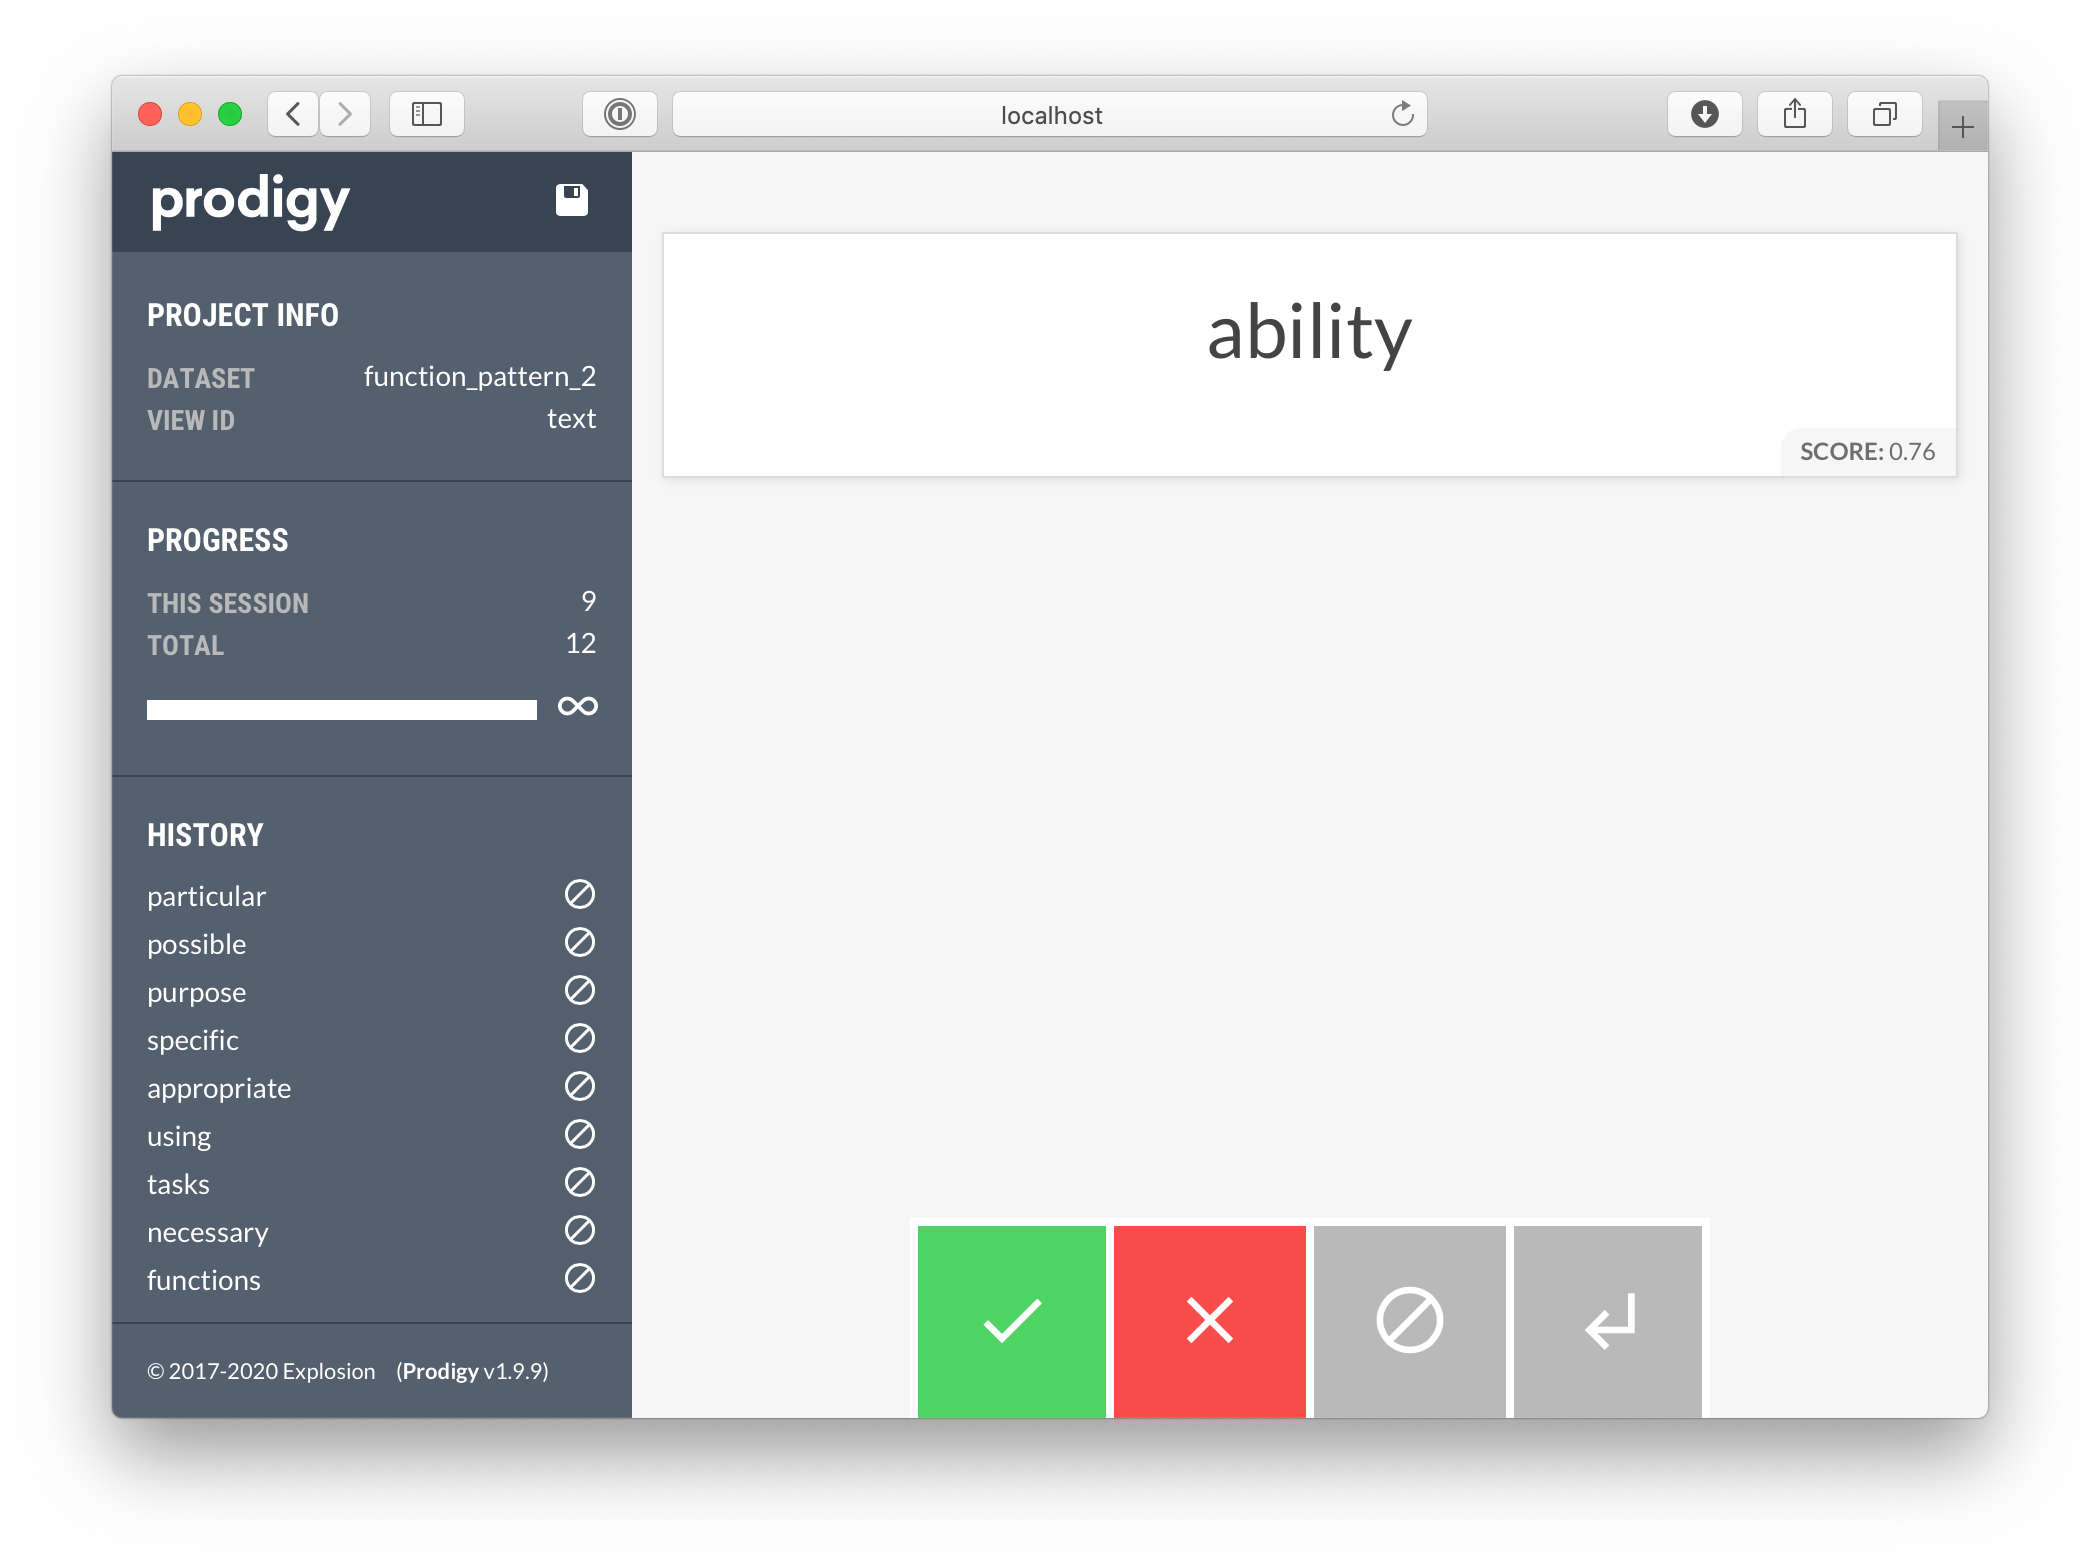
\includegraphics[width=1.19\linewidth]{fig11.png}
  \caption{Prodigy training tool installed in a local developer environment}
  \label{fig:figure11}
\end{figure}
\vspace*{1.2em}

The terms.teach recipe uses word2vec and delivered promising results.
We expected to get better results using sense2vec through the \bverb{textcat.teach} recipe and a new format for seed terms using JSON (a file format for human-readable data objects) instead of plain text.
Seed terms in sense2vec can be initialised using their parts-of-speech, so we can compare results using our focus words as nouns instead other parts that the algorithm identifies in our corpus.
However, we did not get this to work as there are more files required for sense2vec to function.
Simply loading the new seeds as JSON produced errors and loading the seeds from the plain text file assigned verb as a POS for use.
Furthermore, the only corpus that worked out-of-the box with the sense2vec model was Reddit.
Reddit includes the required vectors that are either missing or in a wrong format using \bverb{en\_core\_web\_lg}, making a straight comparison with the word2vec model difficult.

%===================================

\section{Comparison of results}

We compiled results from all above tools into a table (Table \ref{tab:table5}).
From this comparison we can identify certain patterns regarding the context of the words and to an extent understand the effect of a corpus or algorithm on the results.

It can be seen that some words are found in almost every tool while others are unique to a single one.
There are also many repetitions of word stems and lemmas which speaks for poor data preprocessing.

\vspace*{1.2em}
\begin{figure}[!htbp]
  \hspace*{-3.666em}
  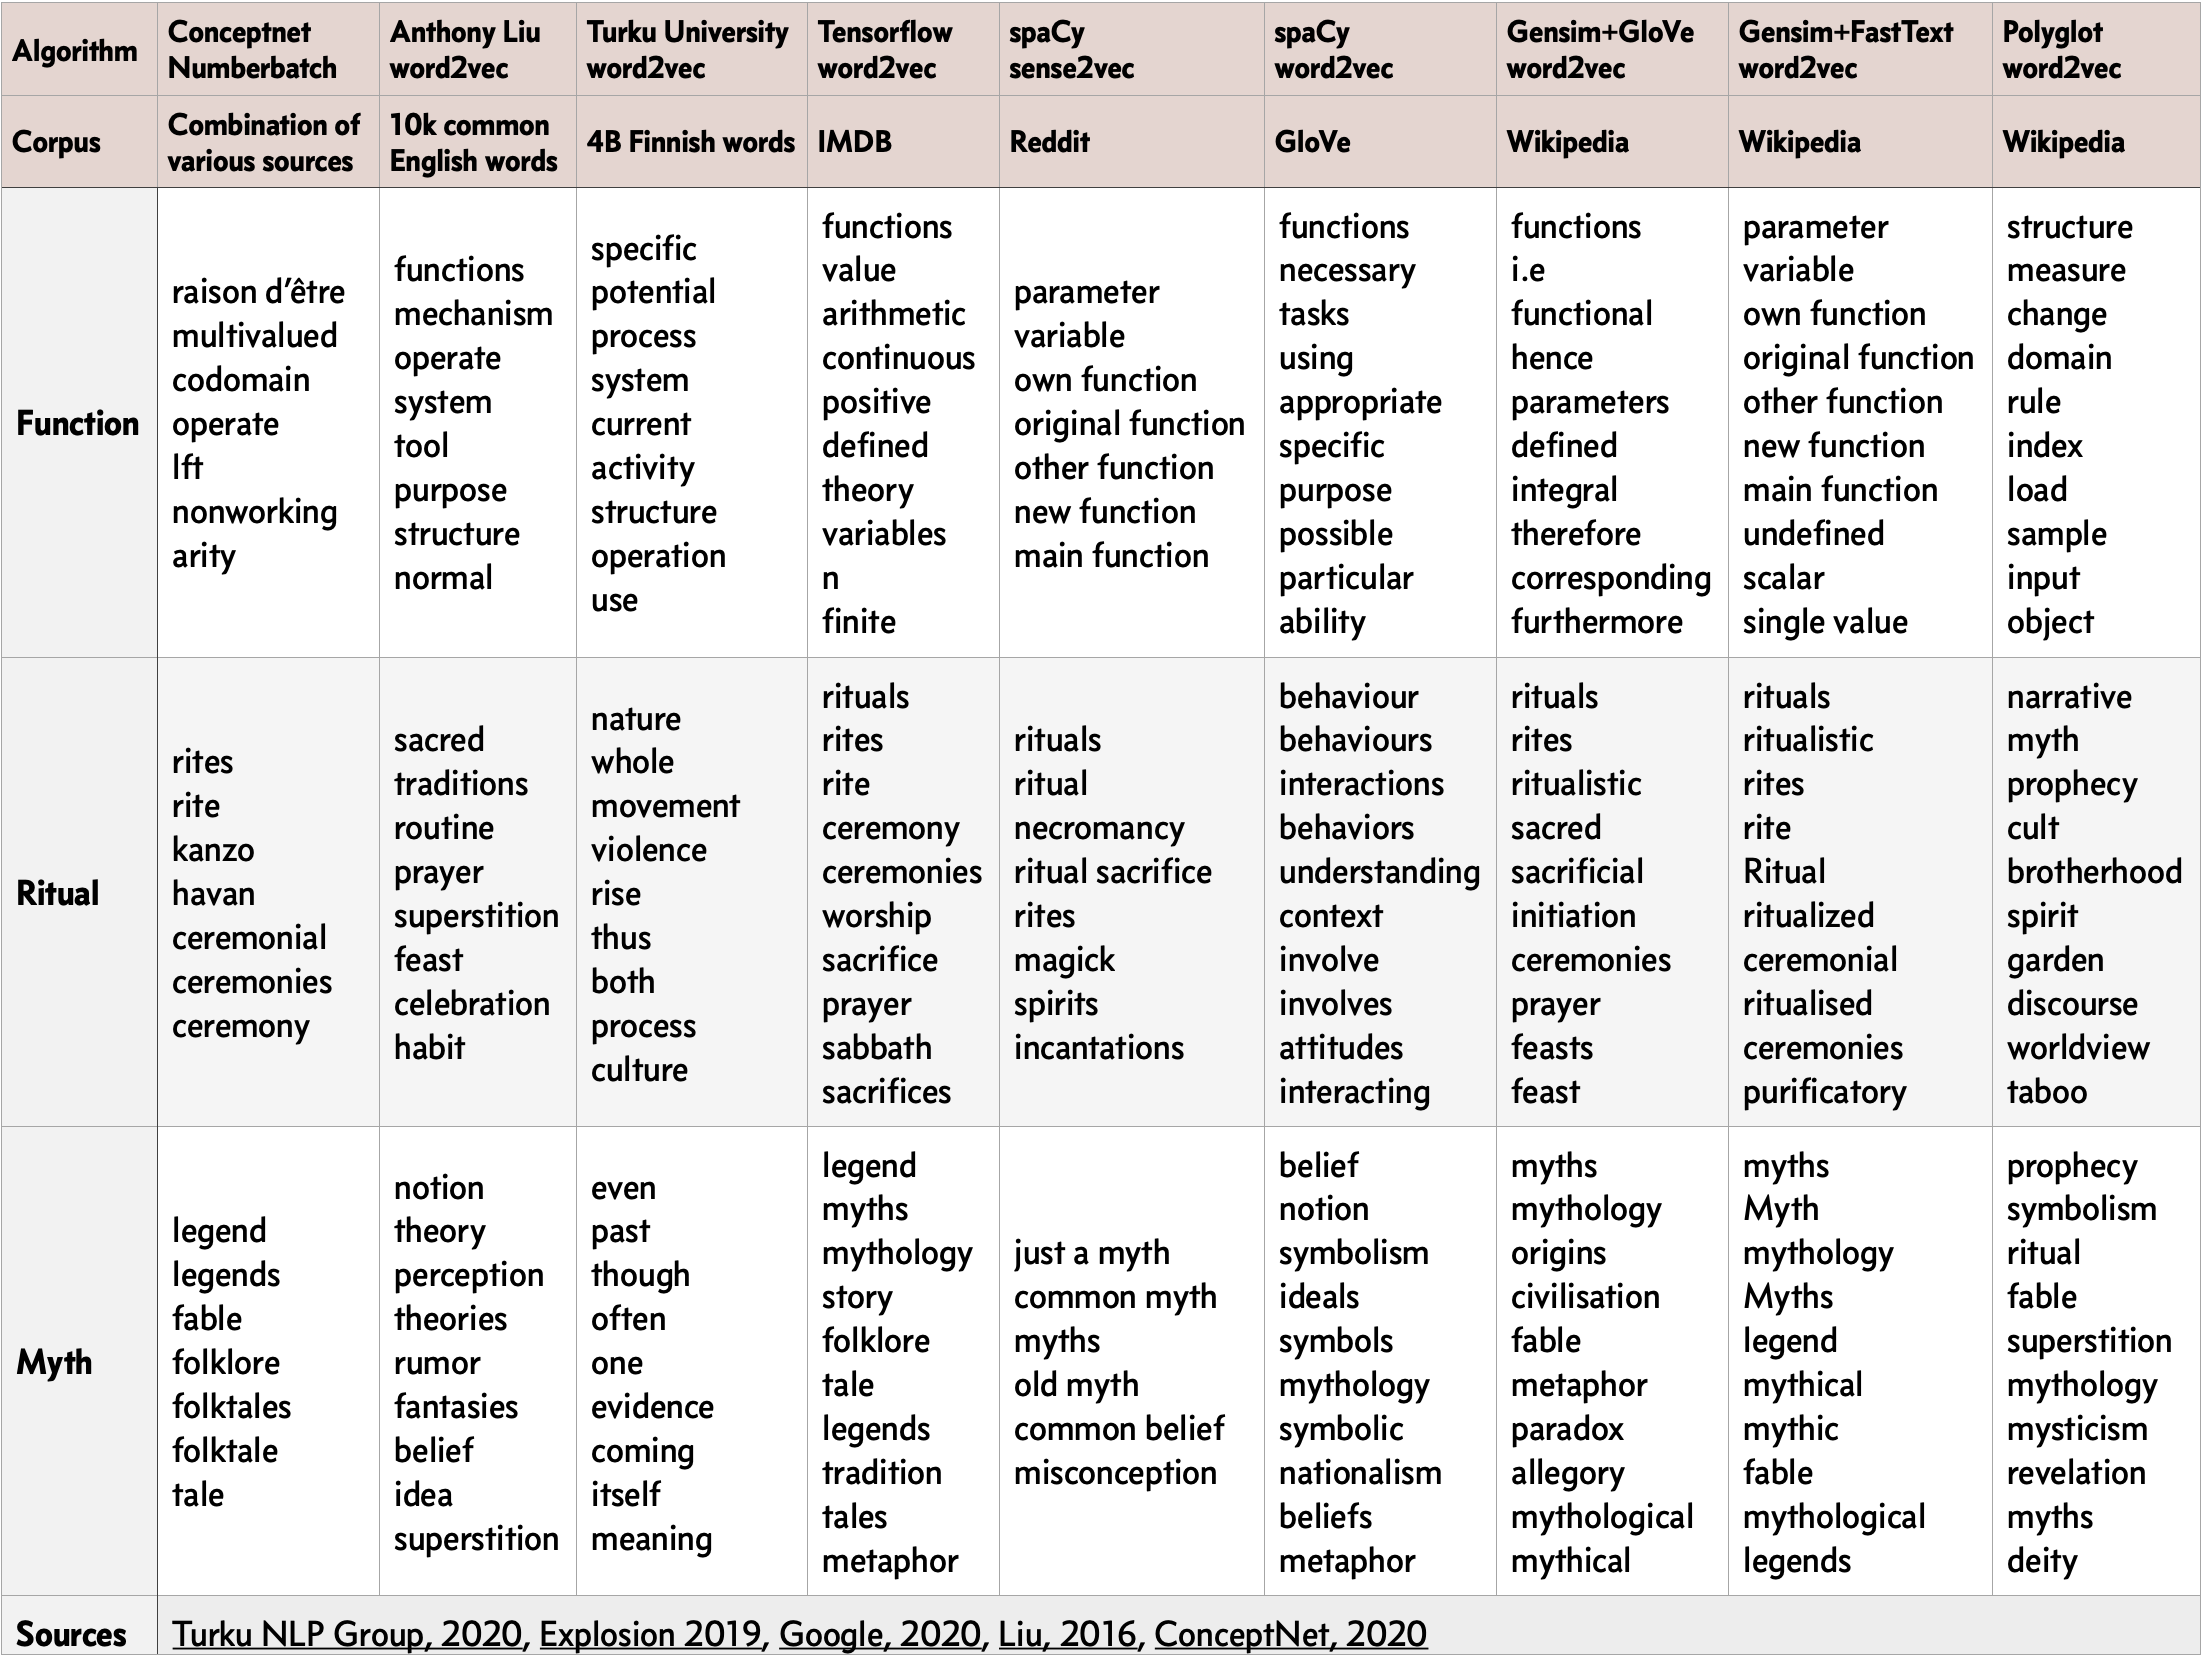
\includegraphics[width=1.19\linewidth]{table5.png}
  \caption{Results from online demos and local scripts using different algorithms and corpora}
  \label{tab:table5}
\end{figure}
\vspace*{1.2em}

Function often exists in the context of computer science, which is not surprising given the field of NLP is one of artificial intelligence, machine learning, data analysis, and formulas.
Parts of computer programs are called functions, and as such we can expect many derivations of the term either as part of a program or just function as the name for a function.
In ConceptNet we can find the word used in the acronym LFT (liver function test) from the field of medicine and arity which comes from mathematics.
It is curious that the IMDB corpus also outputs technical uses of function such as variables or n, which presumably stands for number.
While we do not have exact criteria to rank these results, the output from Polyglot has the most range and fewest repetition of computer science terms.

Ritual was often associated with ceremonial topics and religion.
While there is a certain celebration in the ritualisation of using an object, religion is not the context we intended to evoke.
Tradition, routine and habit found in Anthony Liu’s demo using common English words are more in line with the aspect of social interaction identified by Giacomin (2017) \cite{giacomin2017}.
It can also be observed that spellings of British English and American English are interpreted uniquely, which is in line with the function of word2vec where each morphological structure of a word is assigned their own vector.
We did not sanitise the table by removing these duplicates since they were not identified as such by the machine even though to us they clearly are.
Myth is associated with fairytales, fables, folklore, made-up fantasies and misconception.
Two instances of symbolism can be found in SpaCy with GloVe and Polyglot with Wikipedia.
This finding was interesting as it closes the loop of this document by returning to Susan Fournier’s \ref{fig:function-symbolic} axis of mapping object meanings from functional to symbolic.

%===================================

\section{Current Conclusions}

Regarding our selection of SpaCy paired with Prodigy as the focus, it cannot be ruled out that this combination is still the “winner”, but it is clear that we made mistakes in the application of the tools.
In contrast, the results from the Polyglot demo are the most promising in Table \ref{tab:table5}. 
We have breadth of context without repetitions and are rediscovering symbolism as a potential alternative to myth, which is negatively loaded.

When we used Prodigy with one one seed term (function), the results we saw were exactly the same as those using Gensim+FastText using GloVe.
Both libraries share GloVe and word2vec. Similarity can be expected, a mirror image was surprising.
The results found in Table \ref{tab:table5} are using three seed words.
We also tried 15 seed terms and these were our results: other functions, main function, method, other function, specific function, multiple functions, constraint, certain function.
It is unclear what conclusions we can draw from this.

While there is good documentation available for NLP tools, the field itself is still foreign to us and we have only scratched the surface in understanding the different concepts and are unfamiliar with Python programming.
We focused on Prodigy because it offers text classification and training in a graphical user interface, and put the online demos aside since they are not trained on our context.
In hindsight we should have spent more time looking at the existing demos because we did not achieve the desired training and corpus-comparison using Prodigy.

%===================================

\section{Next Steps}

The combination of Prodigy and SpaCy was interesting to us for one more reason: the trained model can be imported into Tensorflow and visualised in its 3D vector-space.
We did not get to that stage and wish to do this at a later point.
To produce results for the import, we want to revisit ou training and have another the vector files to see if all features (lemmatisation, stemming, polysemy, etc.) are enabled, and to control POS for seed terms.
We also want to try another corpus for training and see if the model finds more diverse and less repetitive results.

The output from Table \ref{tab:table5} will have to be evaluated by non-experts and compared to the dictionary results.

In the next document, we will need to get back to the bigger picture of defining Design for Meaning.
In this publication we focused on NLP and assumed some prior knowledge of the works by Csikszentmihalyi and Rochberg-Halton (1981) \cite{csikszentmihalyi1981}, or more recently by Crilly, Maier, and Clarkson (2008) \cite{crilly2008}, Diller, Shedroff and Rhea (2008) \cite{diller2008} or Gobé (2009) \cite{gobe2009}.

The plan for the next phase of this project is as follows:

\begin{enumerate}
	\item Compare and contrast Table 5 with Table 1 and potentially compile a comprehensive merged version
	\item Build a survey of words to send out to testers and evaluate which words resonate most with people. Get input from people on words that they think are missing from the table.
	\item While waiting on results from the survey, we can have another look at NLP
	\item Re-evaluate the word associations
	\item Build a new survey where we have people classify familiar products into the three categories of meaning, using our new word list.
	\item Evaluate and identify potential patterns
\end{enumerate}

%===================================

\chapter{Phase 2: Contextualisation}

\section*{Introduction}

The weakness of the first stage of our research was a lack of focus.
We did not want to limit our results but the nature of NLP requires some specificity to get good results.
In this chapter, we are introducing context to our research.
We will be explaining more about our rationale later but we decided to be looking at function, ritual and myth in the context of autonomous vehicles (AVs).

The plan written at the conclusion of the first phase needs to be adapted to accommodate for our context.
Here is a revised set of next steps:

\begin{enumerate}
	\item Compare and contrast Table 5 with Table 1 and potentially compile a comprehensive merged version. \emph{Low priority, potentially defer.}
	\item Build a survey of words to send out to testers and evaluate which words resonate most with people. Get input from people on words that they think are missing from the table. \emph{Build a new corpus from various papers.}
	\item While waiting on results from the survey, we can have another look at NLP. \emph{No}
	\item Re-evaluate the word associations \emph{No}
	\item Build a new survey where we have people classify familiar products into the three categories of meaning, using our new word list. \emph{Not products, but attributes of the AV experience}
	\item Evaluate and identify potential patterns
\end{enumerate}

We want to find out what aspects of the AV experience people associate with function, ritual and myth. 
To do that, we will first need to find a common linguistic ground:
What words do people associate with function, ritual and myth?
This time, we conducted surveys with people instead of relying on algorithmic analysis of language. 
With the language established through NLP research as well as individual responses, we can design a survey using words and images that people attach to different meanings.

%todo: replace this image

\vspace*{1.2em}
\begin{figure}[!htbp]
  \hspace*{-3.666em}
  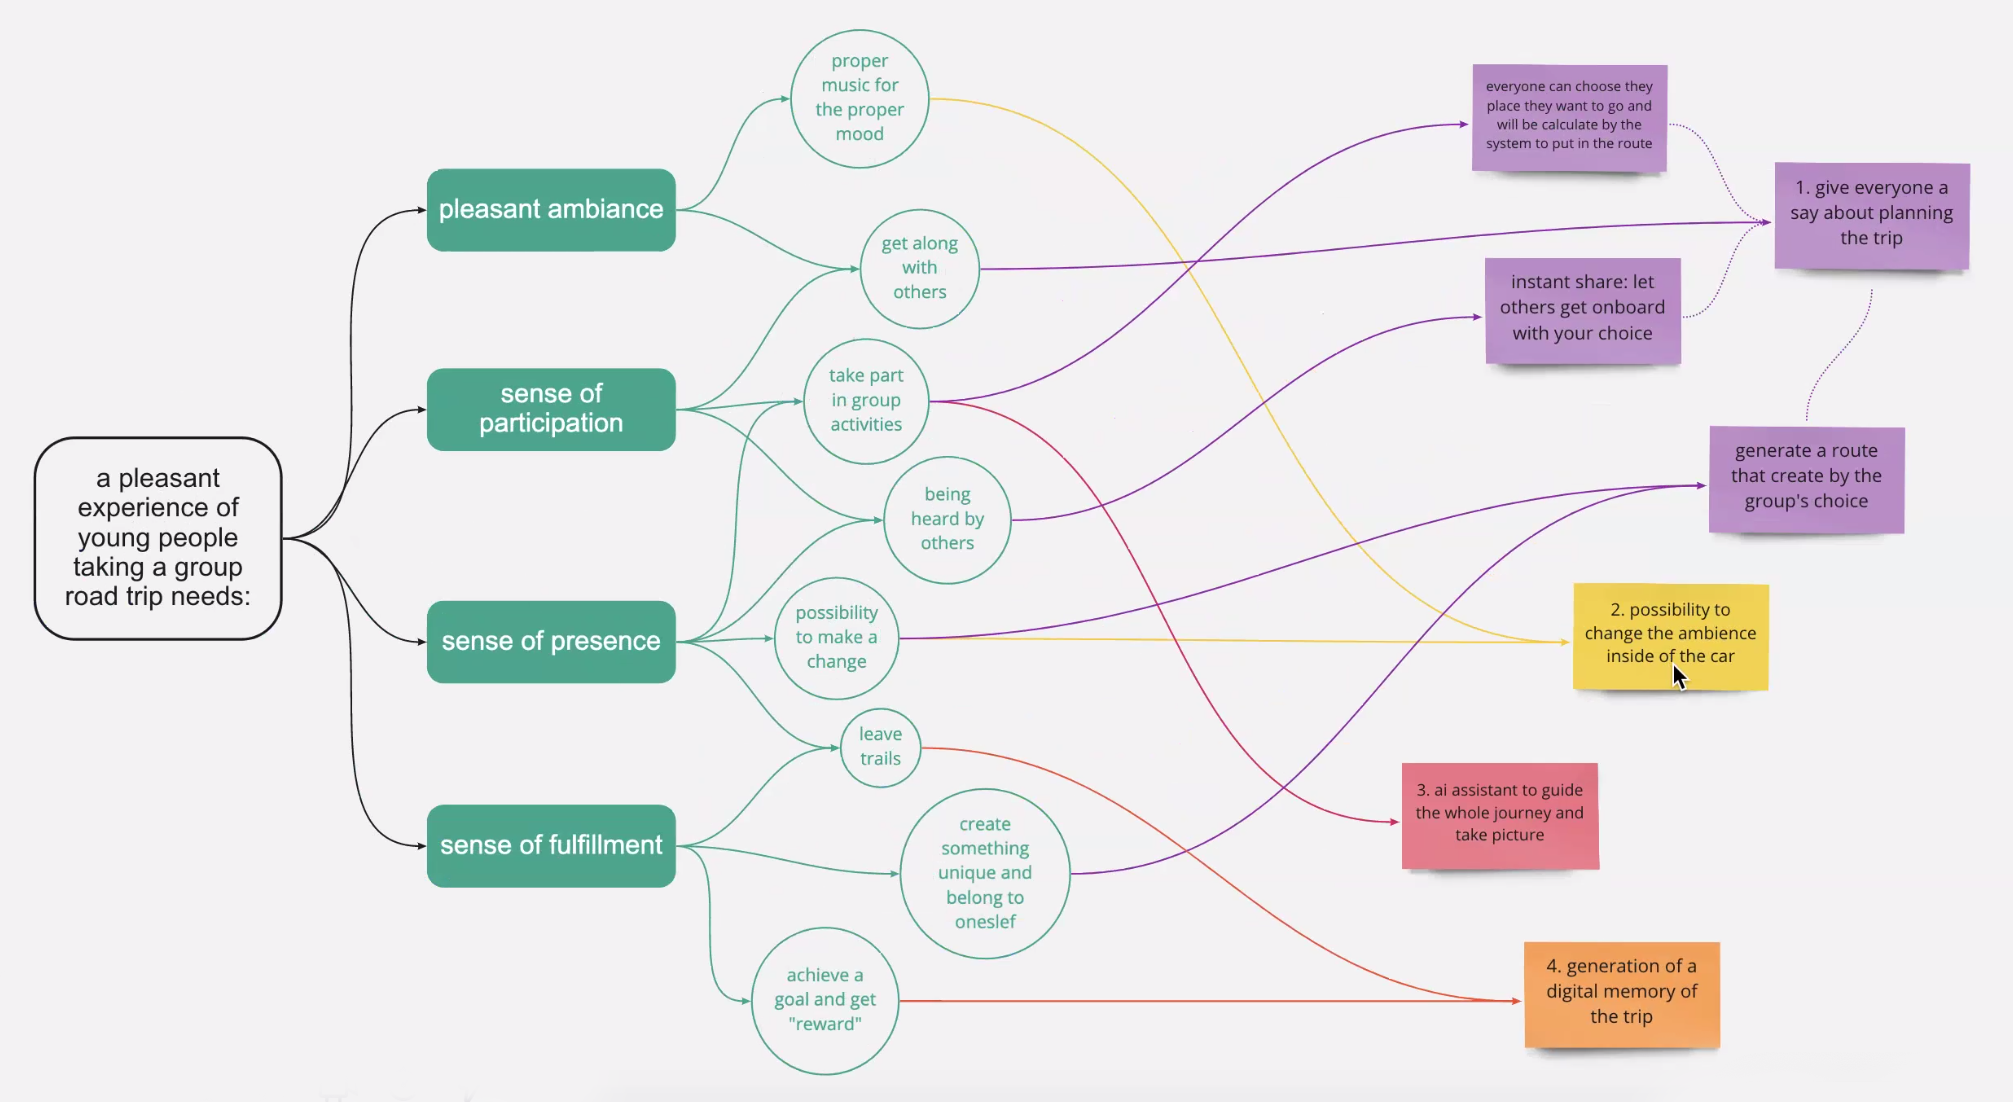
\includegraphics[width=1.19\linewidth]{fig12.png}
  \caption{Metaphors in Cars}
  \label{fig:figure12}
\end{figure}
\vspace*{1.2em}

While AVs have been used since Lawrence and Elmer Sperry's 1916 unmanned air vehicle and industrially as assembly or warehouse robots or military drones (Nonami, 2007) \cite{nonami2007}, their use has not yet emerged for private citizens.
AVs for the public are still only found in driverless trains in airports or Milan's metro system and levels of autonomy in cars, such as cruise control or automatic breaking and parking (Bimbraw, 2015, Duffy and Hopkins, 2013) \cite{bimbraw2015} \cite{duffy2013}. %These techniques are also the enablers for modern technologies of autonomous cars like lane parking, adaptive cruise control, automatic braking, etc (Bimbraw 2015; Duffy and Hopkins 2013). 
The full self-driving consumer car is yet only found in Elon Musk's plans for Tesla's roadmap.
The current main issues with these vehicles is a lack of trust from the general population, as well as unresolved legal and ethical questions about the responsibilities in case of accidents. 
We will go into more detail about these issues in the following \autoref{sec:trust}.

For this chapter, we will first look at our categories in the context of traditional cars, with examples taken from previous research (Giacomin, 2020) \cite{giacomin2020}.
Then, we will shift to the context of AV and see how we can translate our examples, and what attributes can be mapped from traditional to autonomous cars.
Later, we will explain our surveys and discuss results.
Finally, we can debate whether our hypotheses formulated in \autoref{sec:newmetaphors} can be validated.

%===================================

\section{Context: Cars}

The Transport sector is important in various ways.
Economically, the industry accounts for roughly 5 percent of the European workforce and GDP (EU Commission, 2015) \cite{eucom2015}.
Environmentally, the sector accounts for almost a third of greenhouse gas emissions and over 70 percent from that comes from road transport (EEA, 2017) \cite{eea2019}. 
Symbolically, the automobile means freedom.

We tasked four groups of students of the Digital and Interaction Design Master's course at Politecnico di Milano to show the meaning and metaphors used in cars.
Their findings can be seen in the flowchart of Figure \ref{fig:figure12}.

In the following subsections we will have a look at meanings in traditional vehicles. Later, we will shift to autonomous vehicles and look at the new meanings that equivalent products can have. These differences in meaning can potentially inform us of a pattern between existing and new meanings as technology and people's mindset progress.

\subsection{Function}

Mail delivery, garbage disposal, infrastructure inspections \cite{giacomin2020}.

These ways of transport are relevant to our system and while there may be a regularity to these, they are not used in a celebratory way or in a social context. 
The potentially mythical aspect about these is not inherent in the product itself but in the system behind it (for example the postal worker as a symbol does not stem from their vehicle).

\vspace*{1.2em}
\begin{figure}[!htbp]
  \hspace*{5em}
  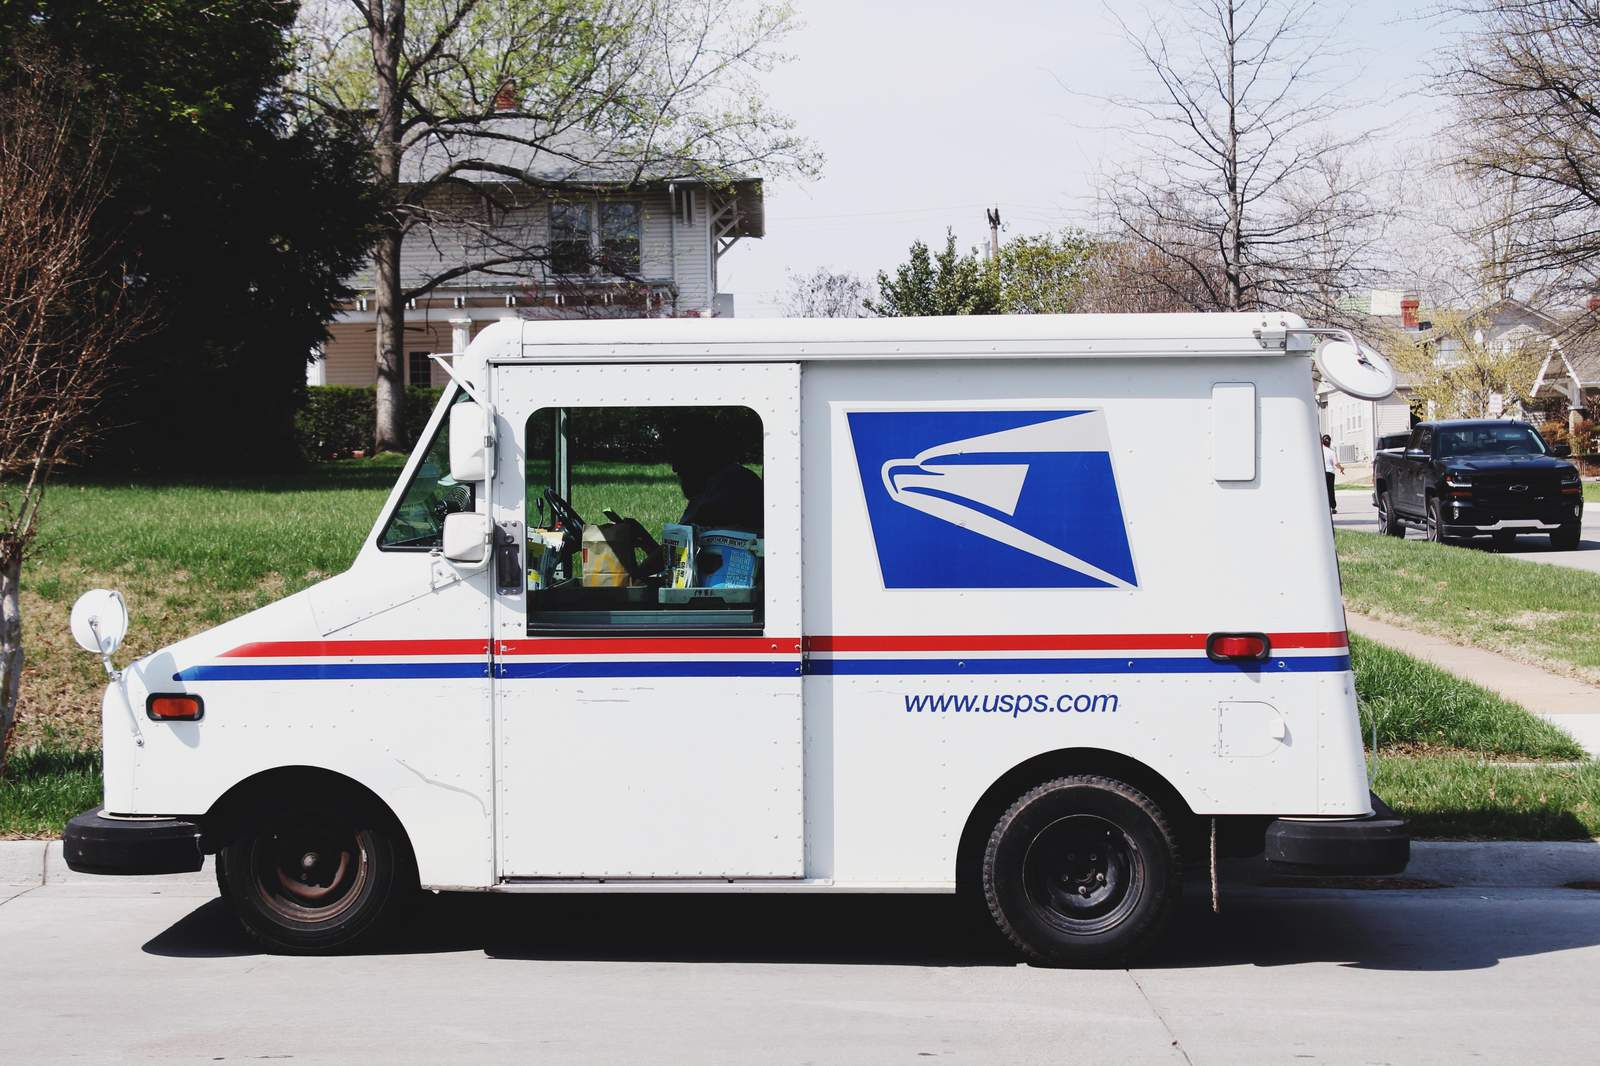
\includegraphics[width=0.7\linewidth]{fig13.jpg}
  \caption{Functional meaning}
  \label{fig:figure13}
\end{figure}
\vspace*{1.2em}

\subsection{Ritual}

The daily commute by bus, car or train \cite{giacomin2020}.
Driving home for Christmas.

These can have functional aspects too, but they also stand for interaction and have an emotional attachment, at least in hindsight.

\vspace*{1.2em}
\begin{figure}[!htbp]
  \hspace*{5em}
  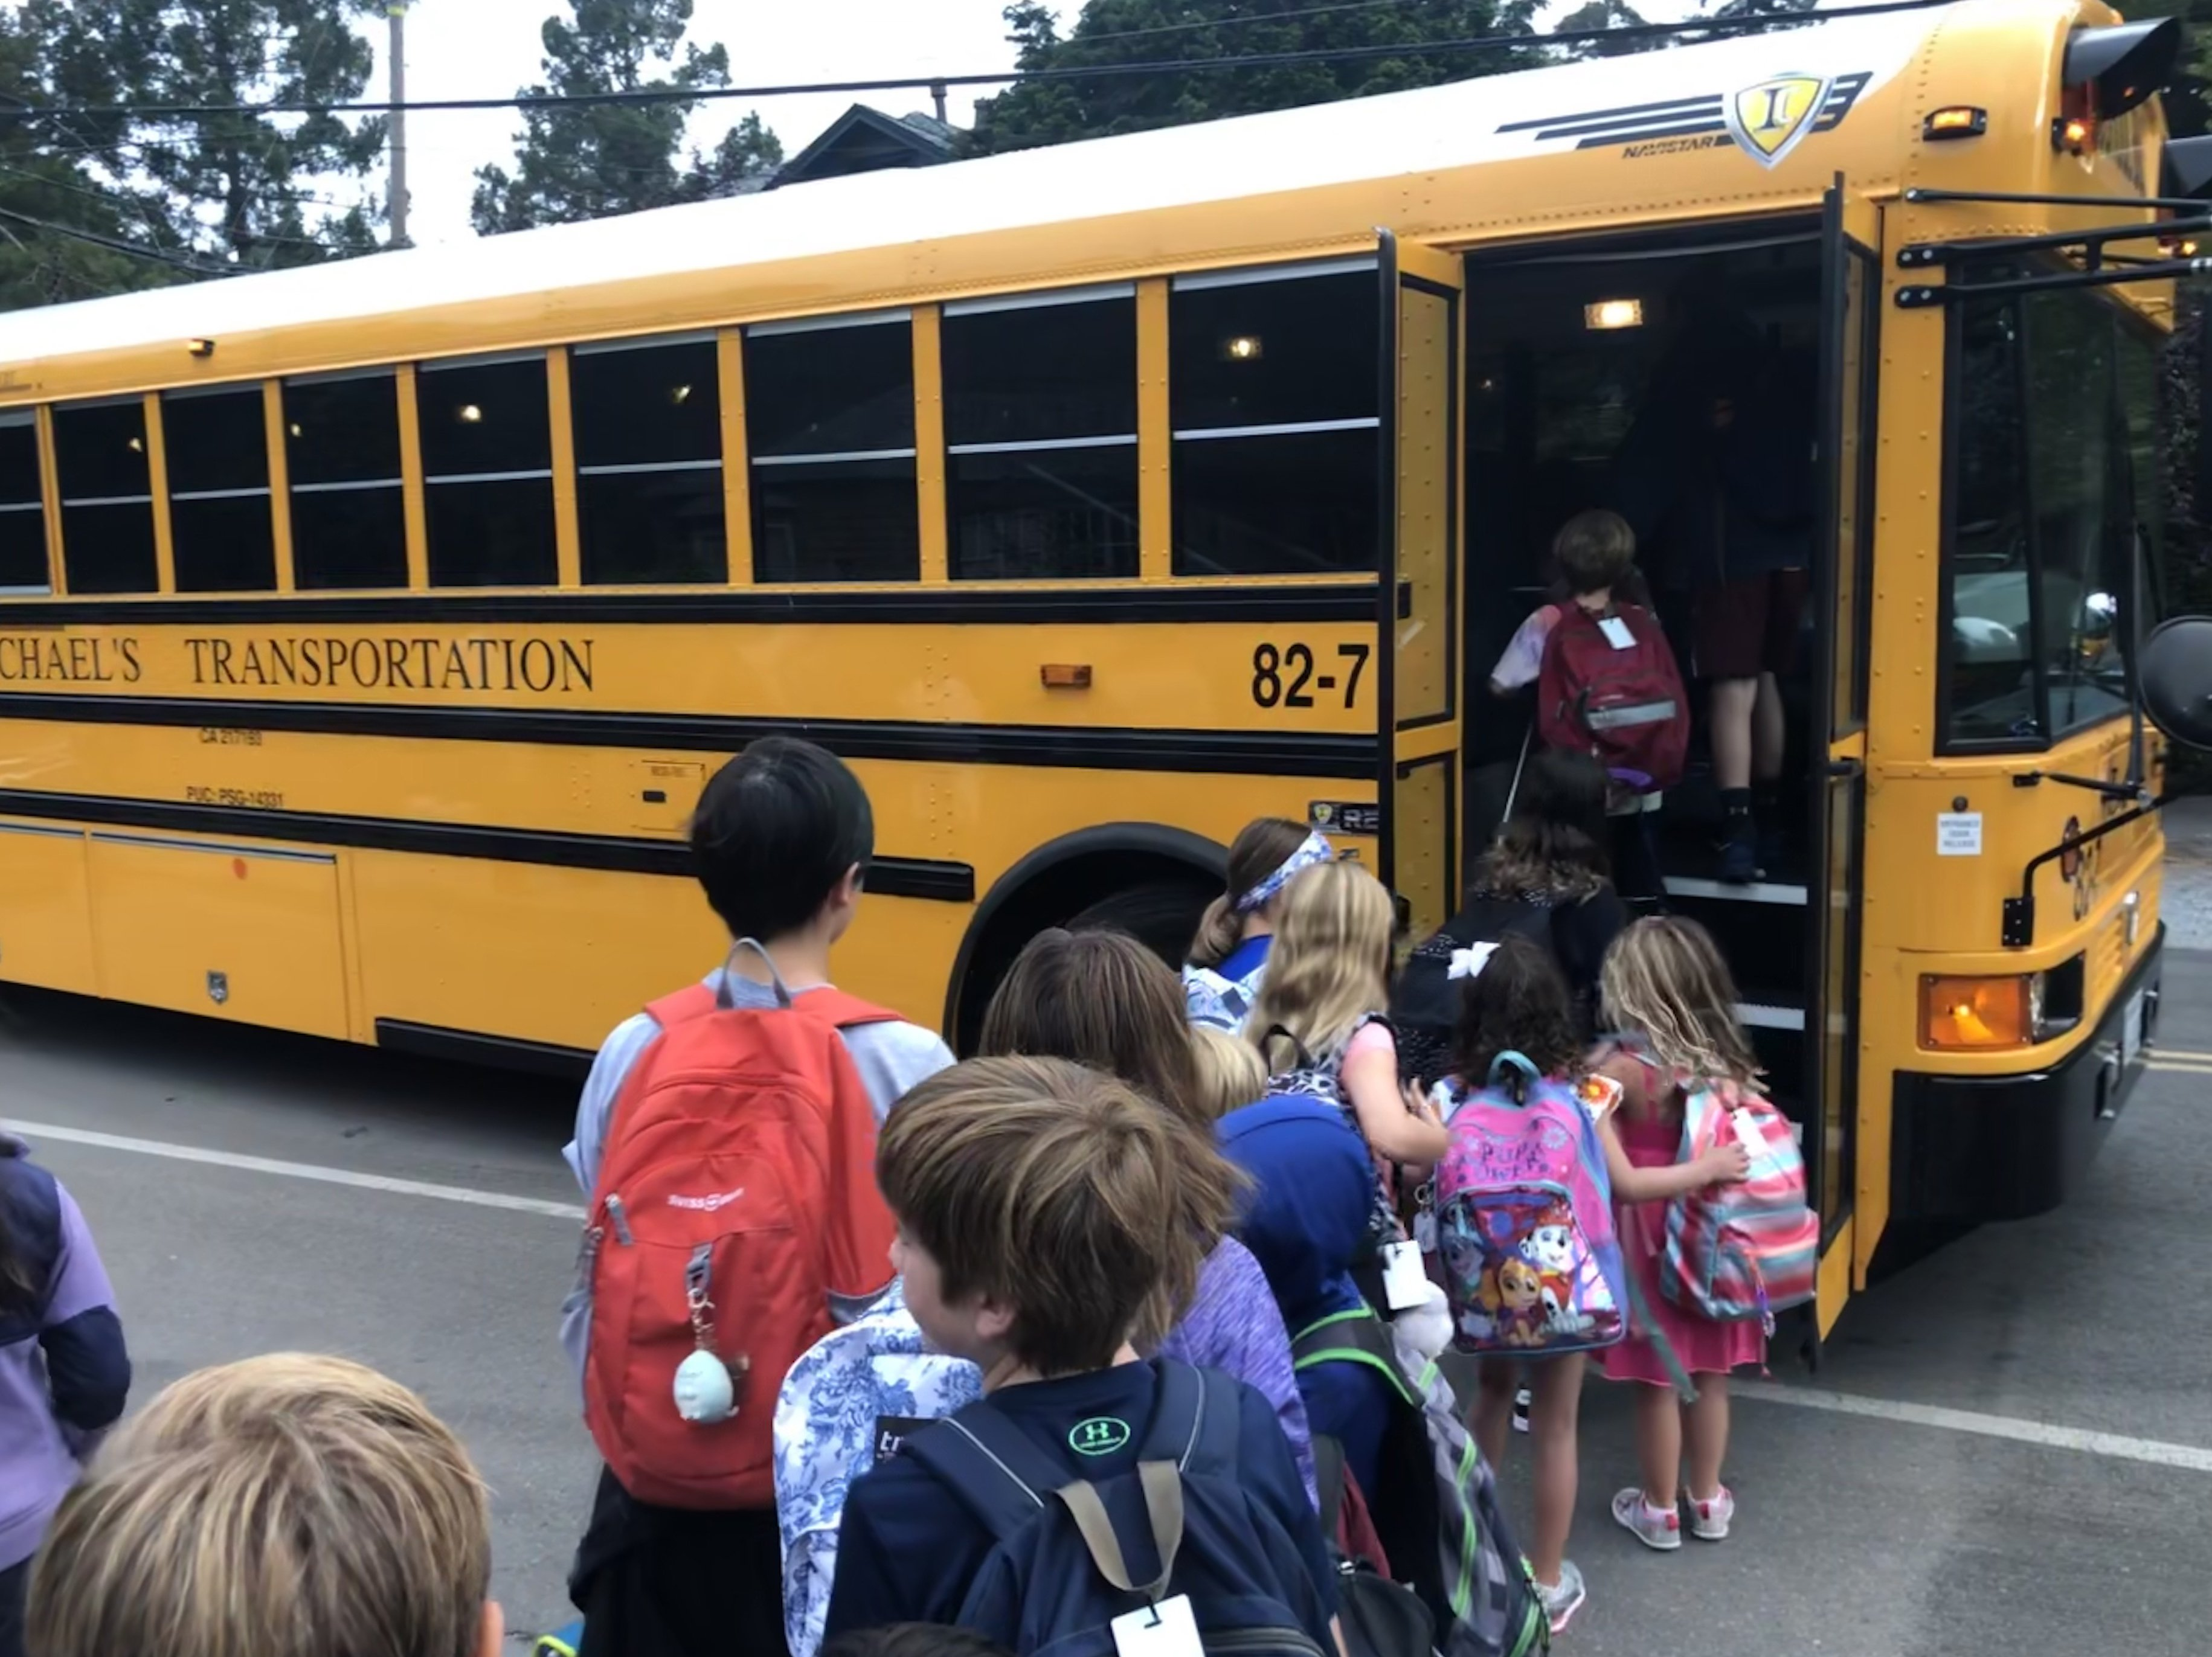
\includegraphics[width=0.7\linewidth]{fig14.jpg}
  \caption{Ritualistic meaning}
  \label{fig:figure14}
\end{figure}
\vspace*{1.2em}

\subsection{Myth}

The aspirational sports-car \cite{giacomin2020}.

\vspace*{1.2em}
\begin{figure}[!htbp]
  \hspace*{5em}
  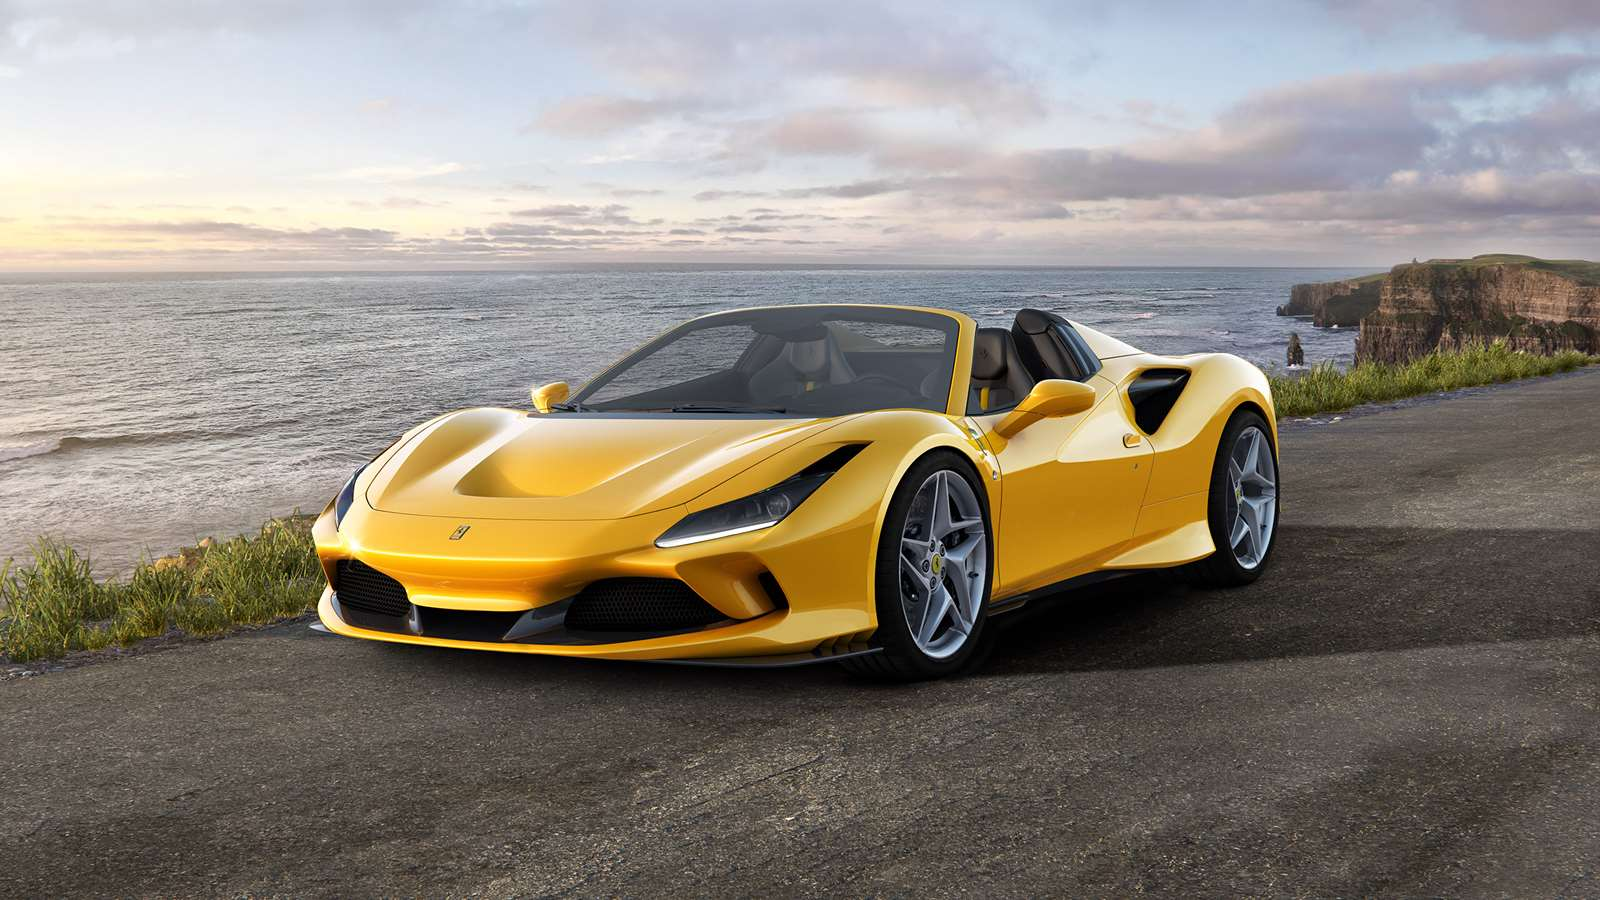
\includegraphics[width=0.7\linewidth]{fig15.jpg}
  \caption{Mythical meaning}
  \label{fig:figure15}
\end{figure}
\vspace*{1.2em}

%===================================

\section{Shifting gears: Automotive Vehicles}

Our methodology to gain insights about people's associations with autonomous cars needs to start by establishing a language we can use to communicate. 
The field of autonomous vehicles is expanding from industrial purposes to public and personal transport and with it the public opinion.
We see the topic as something of not only social but also economic and environmental importance, as the reaching global climate goals depends on collaboration from the industry. 
As such, vehicles and in particular autonomous vehicles are an important global topic, relevant to industry professionals as well as private citizens.

\subsection{Levels of autonomy}

The Society of Automotive Engineers (\href{https://www.sae.org/standards/content/j3016_201806/}{SAE International}) defined the J3016 levels of automation in vehicles, a practise that performs part or all of the dynamic driving task (DDT).
They provided a taxonomy for the six levels from no automation (Level 0) to full driving automation (Level 5) in the context of motor vehicles on roadways \cite{sae2018}. 

Most cars today sit at level 0, where the human performs the DDT but may be assisted by the car in certain ways: emergency braking or warnings in case of line departure or other vehicles in the driver's blind spot.

The lowest level of automation is Level 1, where the car performs some of the driving automatically, such as adaptive cruise control, while the driver still controls steering and braking.
Many cars today also fall into the Level 1 category where the car is capable of steering or acceleration/braking support.

At Level 2 we reach the state-of-the-art in current consumer car features such as Tesla's Autopilot or GM's Super Cruise systems.
This is known as advanced driver assistance systems (ADAS), where the human still monitors the driving environment but the car provides automatic steering, \emph{and} acceleration/breaking support.

Level 3 enters the category of automated driving features, while the previous three levels were driver support features.
Audi's 2019 A8L has a \emph{Traffic Jam Pilot} feature, which allows the car to autonomously drive in heavy traffic up to 60 km/h without any assistance from the driver, alas the feature is awaiting regulatory approval \cite{paukert2018}.
Honda have announced a version of their Legend luxury sedan for 2021 which will also put the car's autonomous features at Level 3 \cite{reuters2020}.
Another candidate for Level 3 would be Tesla's \emph{full self-driving} (FSD) feature.
FSD is a misleading name, as it does not function on every road-type and will require driver intervention at times.
Furthermore, the feature is still in beta-mode, costs \$10.000 to unlock and while technologically impressive, Elon Musk has been promising full self-driving Teslas since at least 2015 \cite{etherington2020} \cite{korosec2015}.
In March of 2020 the company was ranked last for both strategy and execution in the autonomous driving sector \cite{cuneo2020}.

Level 4 is in most definitions full self-driving, limited only by certain rare road conditions.
The car drives itself, even if a human driver does not respond to a request to intervene.
At Level 5, the car is autonomous on all road types.

\vspace{1em}
\begin{table}[h!]
\setlength\extrarowheight{1pt}
\begin{tabular}{@{}>{\raggedright}p{2.5cm}>{\raggedright}p{2.5cm}>{\raggedright\arraybackslash}p{10cm}@{}}
\toprule
Monitoring of the driving environment          & Level of automation       & Description                                                                                                                                                                                                 \\ \midrule
                                           & 0: Driver only            & The human driver performs all aspects of the dynamic driving task.                                                                                                                                           \\ \cmidrule(l){2-3}
                                           & 1: assisted automation    & A driver assistance system performs either steering or acceleration/deceleration, while the human driver is expected to carry out the remaining aspects of the dynamic driving task                         \\ \cmidrule(l){2-3}
\multirow{-5}{*}{Human driver}             & 2: partial automation     & One or more driver assistance systems perform both steering and acceleration/deceleration, while the human driver is expected to carry out all remaining aspects of the dynamic driving task .               \\ \midrule
                                           & 3: conditional automation & An automated driving system performs all aspects of the dynamic driving task (in conditions for which it was designed), but the human driver is expected to respond appropriately to a request to intervene. \\ \cmidrule(l){2-3}
                                           & 4: high automation        & An automated driving system performs all aspects of the dynamic driving task (in conditions for which it was designed), even if the human driver does not respond appropriately to a request to intervene.   \\ \cmidrule(l){2-3}
\multirow{-7}{*}{\parbox{2.5cm}{Automated driving system}} & 5: full automation        & An automated driving system performs all aspects of the dynamic driving task under all roadway and environmental conditions.                                                                                 \\ \cmidrule(l){1-3} 
\end{tabular}
\caption{SAE Standard J3016 - Levels of Automated Driving \cite{sae2018}}
\label{tab:sae-standard}
\end{table}

While these levels are useful in classifying vehicles for industry, for the layperson they are relatively opaque and meaningless.
The differences between levels 3, 4 and 5 are minimal, and the term ``autonomous vehicle'' implies that we can trust the car to make decisions and not that this trust depends on road conditions.
We will therefore refrain from using these classes in our research addressing participants, and simplify the categories to ``traditional vehicle'', ``car with somewhat autonomous features'' and ``fully autonomous car''.

\subsection{Trust}
\label{sec:trust}

Trust happens between people. 
The trust between man and machine relates to the fields of Human-Machine Interaction (HMI) and Human-Computer Interaction (HCI).
There are several papers exploring the issue of trust in AVs such as Häuslschmid and Pfleging, 2017 \cite{haeuslschmid2017}, Bosch and Baumann, 2019 \cite{bosch2019}, or Sweet and Laidlaw, 2020 \cite{sweet2020}.

%todo: elaborate trust subsection
[elaborate...]

\subsection{Ethics}

This factor slows down industrial innovation as the risks are high and boundaries not yet defined.
Some car manufacturers are shying away from automation as their income lays in traditional cars and they do not want to damage their cash cow.
Ironically, holding on to what is proven to work is not a universal recipe for success and rather leaves room for real innovators to swoop in and take a share of the profit.

%todo: elaborate ethics subsection
[elaborate...]

%===================================

\chapter{New Metaphors}
\label{sec:newmetaphors}

\section*{Introduction}

We identified one iconic example per category of Function, Ritual and Myth for traditional vehicles, but how do the meanings map to autonomous cars?
What does the mail delivery vehicle look like in the context of AV? 
Are the attributes of \emph{aspirational} and \emph{self-driving} compatible in a sports car?
If not, what qualities lie within a fun autonomous vehicle we look at longingly?
We aim to answer these questions in the following sections.

These following three sections aim to convert Giacomin's work (2020) \cite{giacomin2020} from the context of traditional vehicles to autonomous cars, including the challenges in the tasks of these cars.

%===================================

\section{Function: Mail Delivery}

The global distribution chain is already a largely automated organism. 
The main involvement of humans is in last-mile delivery:
Getting items from the distribution center to the door \cite{mckinsey2016}.
Delivery companies use vans and human drivers, who also bring the mail to the recipient's door.
This leaves the van parked on the road for extended periods while the delivery person makes their way through a multi-story residential block.
In large cities such as New York, where more than 1.5 million packages are delivered daily, leaving vans double-parked on the street plays a large role not only in congestion and emissions, but also puts infrastructure to its limits.
Delivery vehicles are stopping in driveways, on bike lanes, and have in 2018 collected over \$27 million in fines \cite{haag2019}.

\vspace*{0.8em}
\begin{figure}[!htbp]
  \hspace*{5em}
  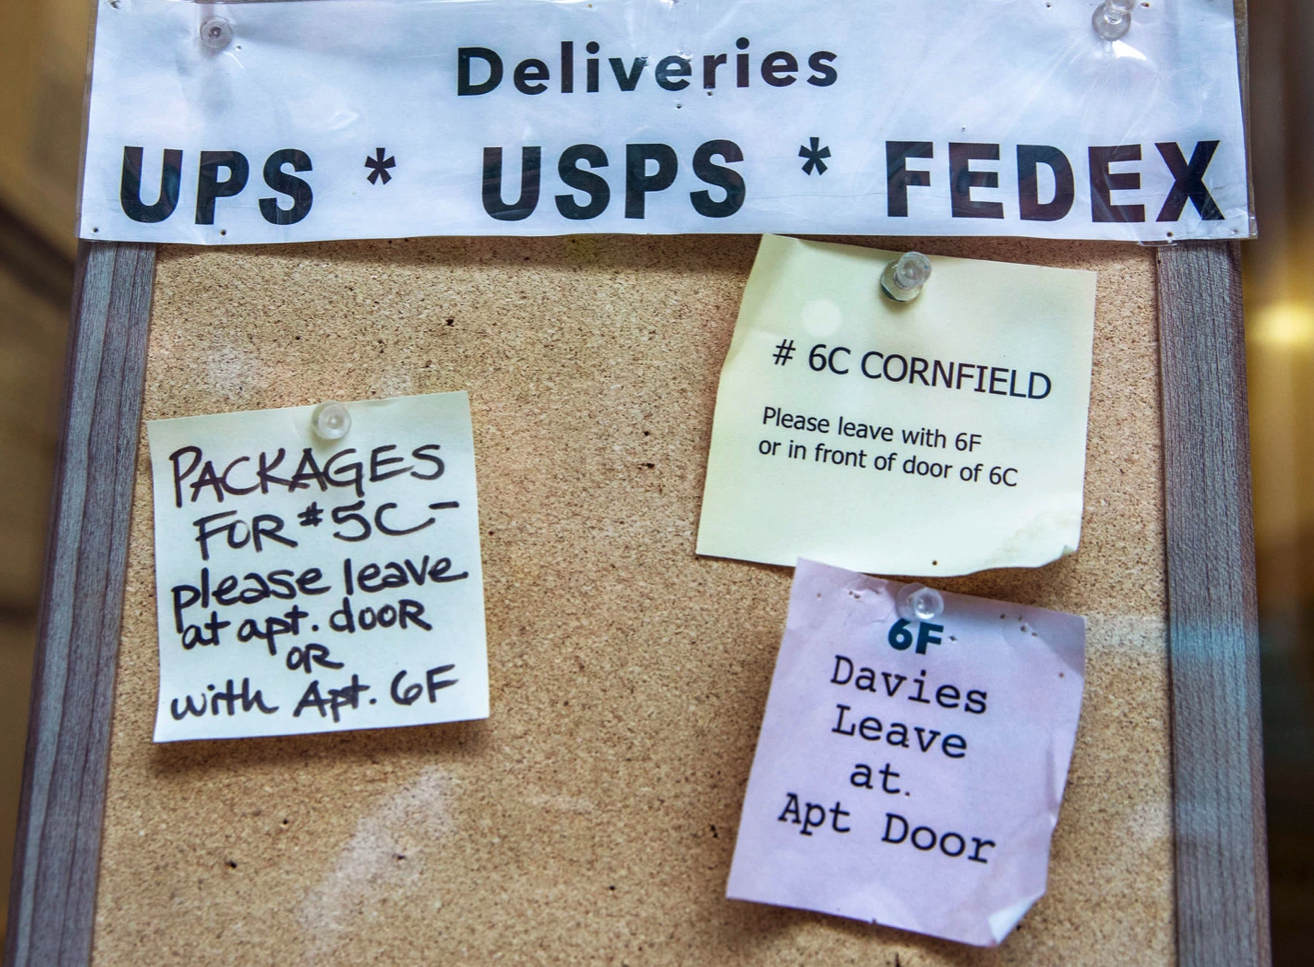
\includegraphics[width=0.7\linewidth]{Brittainy Newman - NYT.png}
  \caption{In congested cities there are many edge-cases which make it difficult for AVs to predict situations. Image credit: Brittainy Newman / New York Times (cropped to fit)}
  \label{fig:newmannyt}
\end{figure}
\vspace*{0.6em}

From 2009 to 2017 the average amount of deliveries to households tripled to more than 1.1 million.
In 2020, with online-orders reaching new highs, there seems to be no sign of that trend slowing down.

In an interview with The New York Times \cite{haag2019}, Sarah Kaufman, associate director of the Rudin Center for Transportation Policy and Management at New York University, spoke about a study on online shopping habits she worked on.
“It’s now cheaper and easier to order anything online than it is to go to the store.
We’ve entered an entirely new way of buying goods and services, but our infrastructure is only adapting incrementally, we need to completely rethink how we use our streets if we want to maintain our current shopping and delivery habits.”, Ms. Kaufman said.

A paradigm shift in the vehicles occupying our cities can therefore be a valid attempt at addressing the issues surrounding traffic, pollution, noise and stress.
We can help citizens and delivery companies, but employees of delivery companies might need retraining from driver to supervisors of AVs.

McKinsey (2016) \cite{mckinsey2016} have identified seven delivery models looking at around 300 start-up companies in the last-mile sector and reviewing over 2.000 published articles about new technologies: 

\begin{enumerate}
	\item Today's traditional model of dedicated delivery person with a van, employed by the parcel delivery service provider, bringing parcels from a delivery base directly to the recipient.
	\item Semiautonomous ground vehicles, using an AV but requiring a human driver for handoff and car supervision.
	\item Autonomous ground vehicles (AGV), a mobile parcel locker without human intervention, with one central remote supervisor per eight AGVs.
	\item Flying drones carrying parcels to their destination along the most direct air route with one supervisor per eight drones.
	\item Ground droids --- small AVs the size or a larger parcel using the sidewalk, traveling roughly at walking speed, with one supervisor per 50 to 100 due to small size and low speed.
	\item Crowdsourcing, creating flexibility in supply, is a low investment for parcel delivery companies.
	\item Bike couriers employed by the companies, carrying a small number of letters and parcels.
\end{enumerate}

While the future of Amazon orders arriving via drone within minutes may still be science-fiction, it's not unreasonable to envision a combination of autonomous driving technology and human assistance --- after all, that space is already occupied by certain consumer cars today \cite{mcfarland2020}.

The context of autonomous vehicles allows us to remove the human component from the equation:
We can compare cars and their capabilities. 
From the McKinsey study \cite{mckinsey2016} the models that allow for the closest comparison are models 2, 3, 4 and 5.
Model 2 is very similar to today's model 1.
McKinsey identify a high cost to implement autonomous delivery vehicles and do not see a large enough return on that investment if people are still required for final hand-off and supervision.
Therefore, we can disregard model 2.
Models 3, 4 and 5 can be classified:
While 4 and 5 are for transport of individual parcels (or small amounts) going to individual addresses, the AGV is designed for mass-transport for a collection of addresses.
Whether these vehicles stop at a street corner and demand recipients to collect their parcel or they stop at people's doorstep, these robots won't hand over the parcel.
It seems like model 3 will be asking more from the recipient in the global distribution chain.
We are then left to speculate how the mail delivery will work for those with a walking disability, even a temporary one such as a broken ankle or a cold forcing them to remain in bed.
Will these people rely on the kindness of their neighbours or will the delivery services provide a more flexible, human delivery person for edge cases?

The most likely contender then seems to be a ground droid capable of climbing stairs, as flying drones would not fare well in staircases.
Perhaps the last-mile delivery method of the future is not one smart robot or a mobile locker but a combination of fast vehicles traveling through main streets and hyper-local AVs not for the entire last mile but merely the last metres. 

%===================================

\section{Ritual: Commuting}

%todo: elaborate new metaphor for ritual
[elaborate...]

%===================================

\section{Myth: The fun car}

%todo: elaborate new metaphor for myth
[elaborate...]

%===================================

\chapter{Surveys}

Initially, we relied on literature reviews to gain knowledge about function, ritual and myth.
We found that gathering larger amounts of information introduced some objectivity as we had to make assumptions and decisions on strategy. 
Instead, at this stage we decided to interview people, or rather we built interactive surveys that we could send to people to have them fill out safely in their homes.

To test how people understand function, ritual and myth we first conducted a semantic quantitative survey and later, using the learnings from this survey, a more qualitative test in the context of the autonomous vehicle.

%===================================

\section{Survey 1: Word Meaning}

\vspace*{1.2em}
\begin{figure}[!htbp]
  \hspace*{-3.666em}
  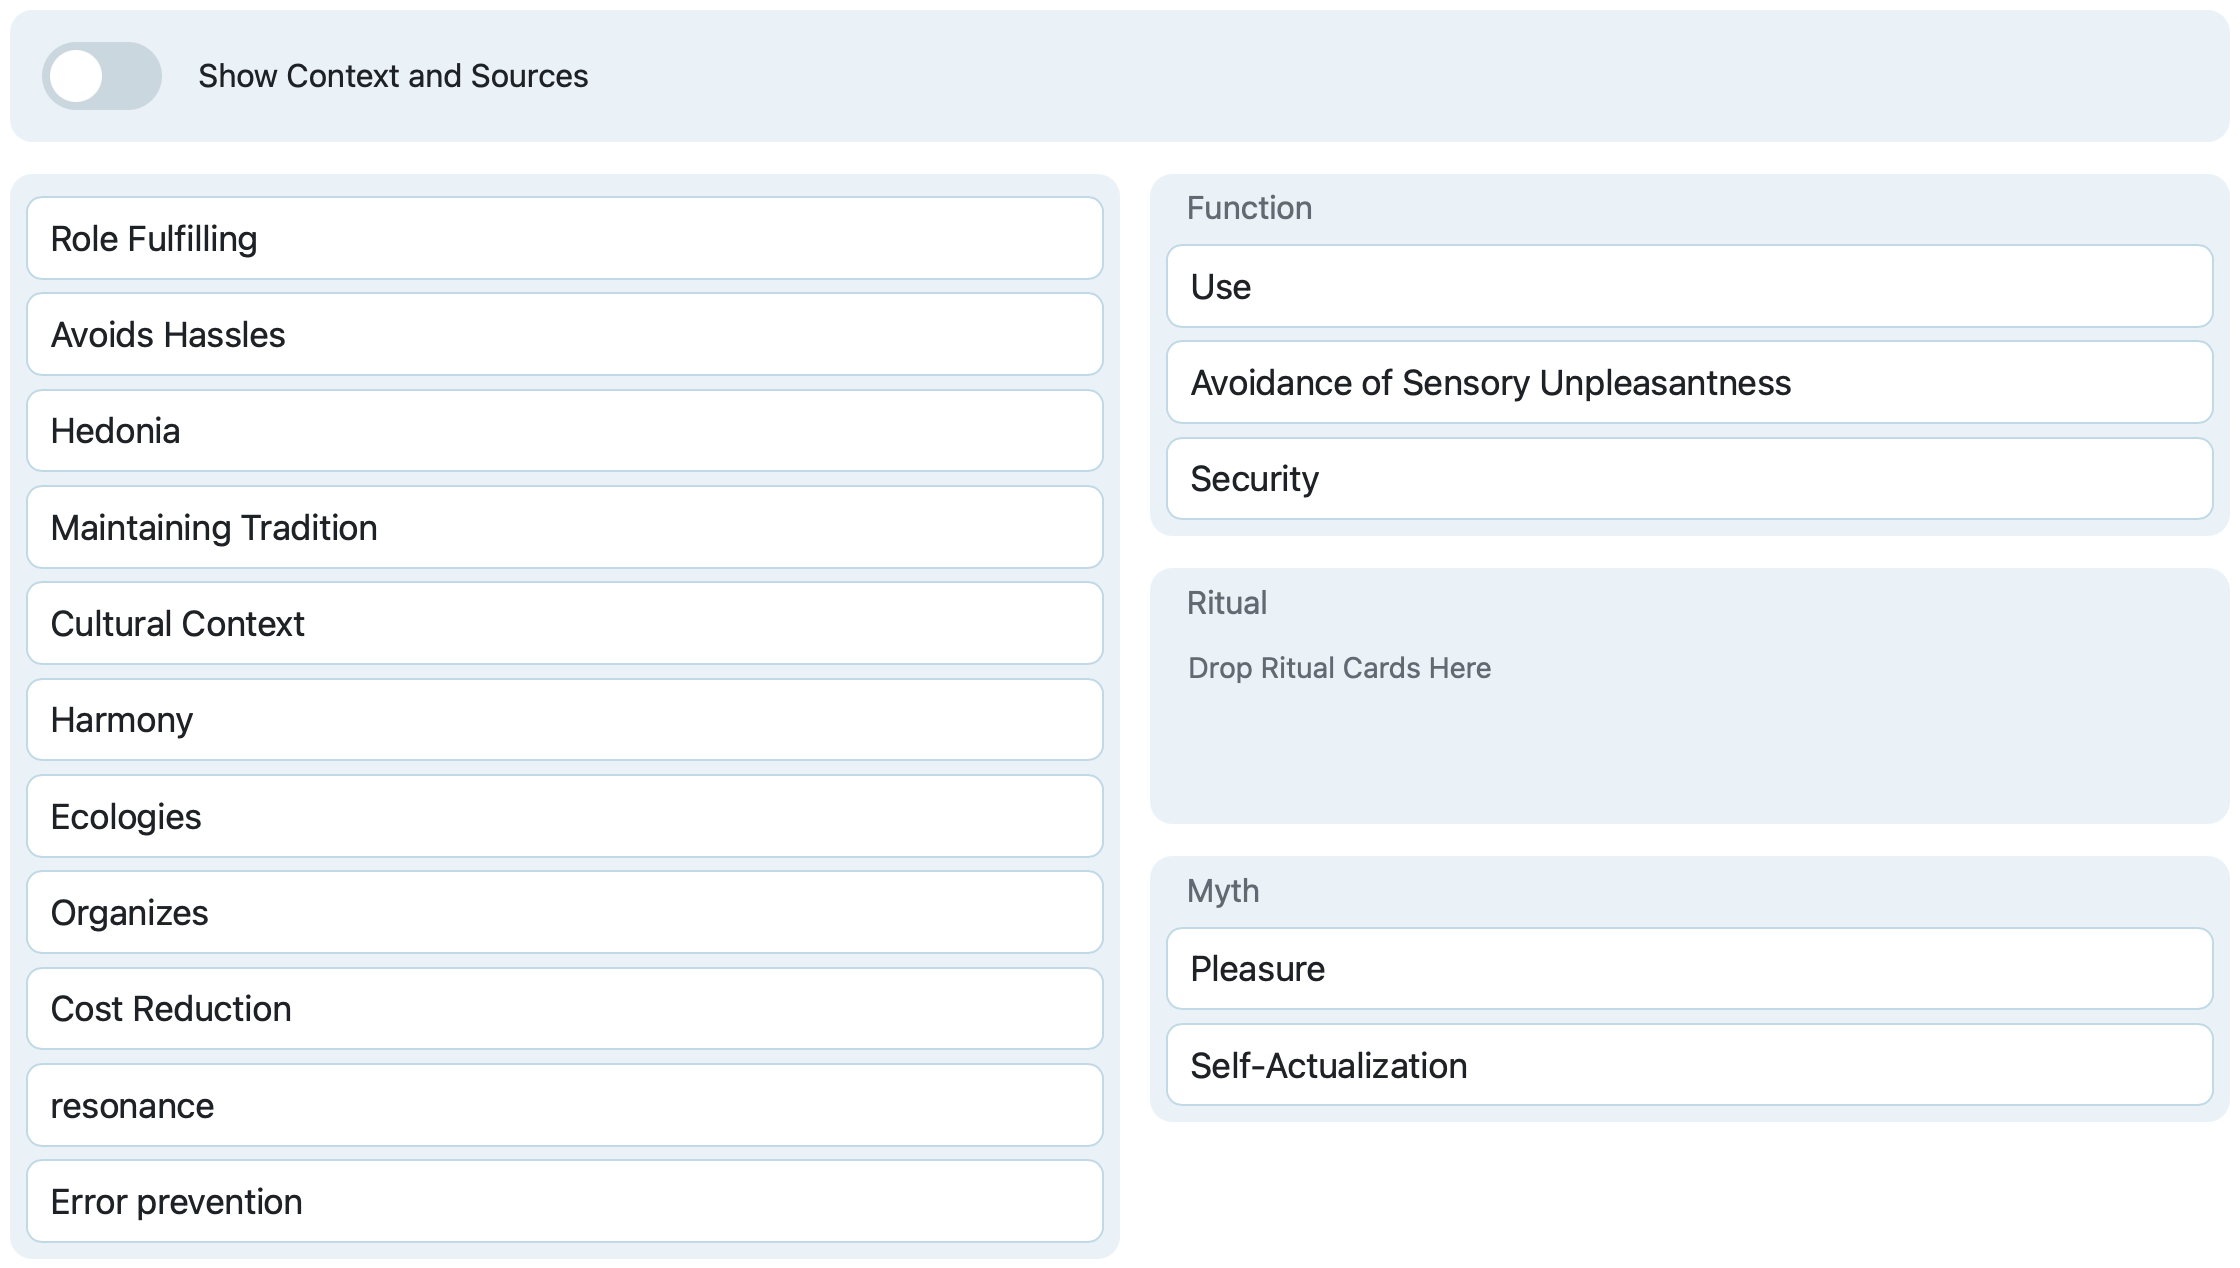
\includegraphics[width=1.19\linewidth]{fig16.png}
  \caption{Word association survey on our \href{https://meaning.pub}{website}}
  \label{fig:figure16}
\end{figure}
\vspace*{1.2em}

This survey was designed and developed for the purpose of collecting words from 12 selected papers on meaning. 
We marked 105 words of phrases from the papers and tasked our survey-takers with classifying them into the rubrics of function, ritual and myth in batches of 16.
We did not want testers to sort 105 words, so we broke it down into random samples and invited people to do the survey multiple times to cover more words.
Results were saved into a table and we were able to analyse the frequency of each term appearing per category.
The random nature of the sortable words meant that fewer votes for a word can mean that these words were skipped because participants were confused by them, or that these words were more rarely displayed.
In the end, the difference is negligible as a word that often appears within a given category and never appears in another is a clear signifier for that word's association.
Ambiguous results should be left unclassified and moved to a ``undetermined'' category.
While they will not be sorted, the raw data is still potentially useful.

The survey was sent out to friends, colleagues and students of Politecnico di Milano and Brunel University London.
Between September 26th and December 14th 2020 we received 140 answers to the survey with 667 votes for Function, 557 for Ritual and 439 for Myth.

%===================================

\subsection{Results}

\vspace{1em}
\begin{table}[h!]
\setlength\extrarowheight{1pt}
\begin{tabular}{@{}>{\raggedright}p{5cm}>{\raggedright}p{5cm}>{\raggedright\arraybackslash}p{5cm}@{}}
\toprule
Function (41 Terms)         & Ritual (26 Terms)      & Myth (18 terms)                                                                                                                                                                                                 \\ \midrule
Interaction, 
Purpose, 
Goal, 
Use, 
Language, 
Life Cycle, 
Security, 
Saves Time, 
Simplifies, 
Makes Money,  
Reduces Risk,  
Organizes, 
Reduces Effort,  
Quality, 
Informs, 
Design, 
Wellness, 
Provides Access,  
Competence, 
Autonomy,
Physical Health, 
Security, 
Self-actualization, 
Utilitarian Value,
Body Language,
Time Management, 
Accessibility,
Physical Compatibility, 
Safety,
Performance and Efficiency,
Durability and Reliability,
Use Economy,
Visibility of System Status,
Match between system and the real world, 
User control and freedom,
Consistency and standards,
Error prevention,
Flexibility and efficiency of use, 
Aesthetic and minimalist design, 
Help users,
Help and documentation

& 

Connectedness,
Accomplishment,
Creation,
Community, 
Duty,
Enlightenment, 
Harmony, 
Oneness,
Truth,
Validation,
Integrates,
Cost Reduction,
Variety,
Reduces Anxiety,
Rewards Me,
Therapeutic Value,
Self-Actualization,
Popularity,
Purchase Economy,
Face Saving Acts,
Impression Management,
Group Belongingness,
Maintaining Tradition,
Memorability,
Surprise,
Recognition rather than recall

& 

resonance,
Significance,
Cultural Context,
Beauty,
Freedom,
Wonder,
Sensory Appeal,
Nostalgia,
Attractiveness,
Provides Hope,
Affiliation,
Self-esteem,
Money,
Interpersonal Ties,
Self-Expression,
Good Luck,
Eudaimonia,
Hedonia

                                                                               
\\ \midrule
\end{tabular}
\caption{Results from Survey 1}
\label{tab:survey1-results}
\end{table}

Some terms received equal votes for each category, and others only differed by a single vote. 
We defined a clear winner by having a lead of at least two votes.
Arguably, this lead is not enough and we may revisit the definition of a winner in the future.
Some terms are over 90 percent in one category while others are a closer call.

Until we determine a better definition for a winner, the undetermined terms remain: 
Coherence,
Ecologies,
Justice,
Redemption,
Connects,
Avoids Hassles,
Badge Value,
Fun,
Motivation,
Heirloom,
Relatedness,
Pleasure,
Enjoyment,
Appropriateness,
Sensory Unpleasantness,
Role Fulfilling,
Affection,
Fun,
Serenity,
Comtemplativeness.

We made a mistake in creating the survey and repeated the term ``fun'', we did not decide to tally up the results for both instances since one of the entries is tied 7 votes per category, and the other one only leads by one point for the category of Function.

\subsection{Conclusion}

To summarise Survey 1, we now know which terms people clearly associate with each of our three categories, and we also know the more ambiguous terms which we should avoid as they might confuse people.

People seem more confident in determining words as Function (39 percent of the terms) than they are for the other two categories (25 and 19 percent respectively), and almost a fifth of our terms (19 percent) remain unclassified.

%===================================

\section{Survey 2: Relevance to Autonomous Vehicles}

\vspace*{0.5em}
\begin{figure}[!htbp]
  \hspace*{-3.666em}
  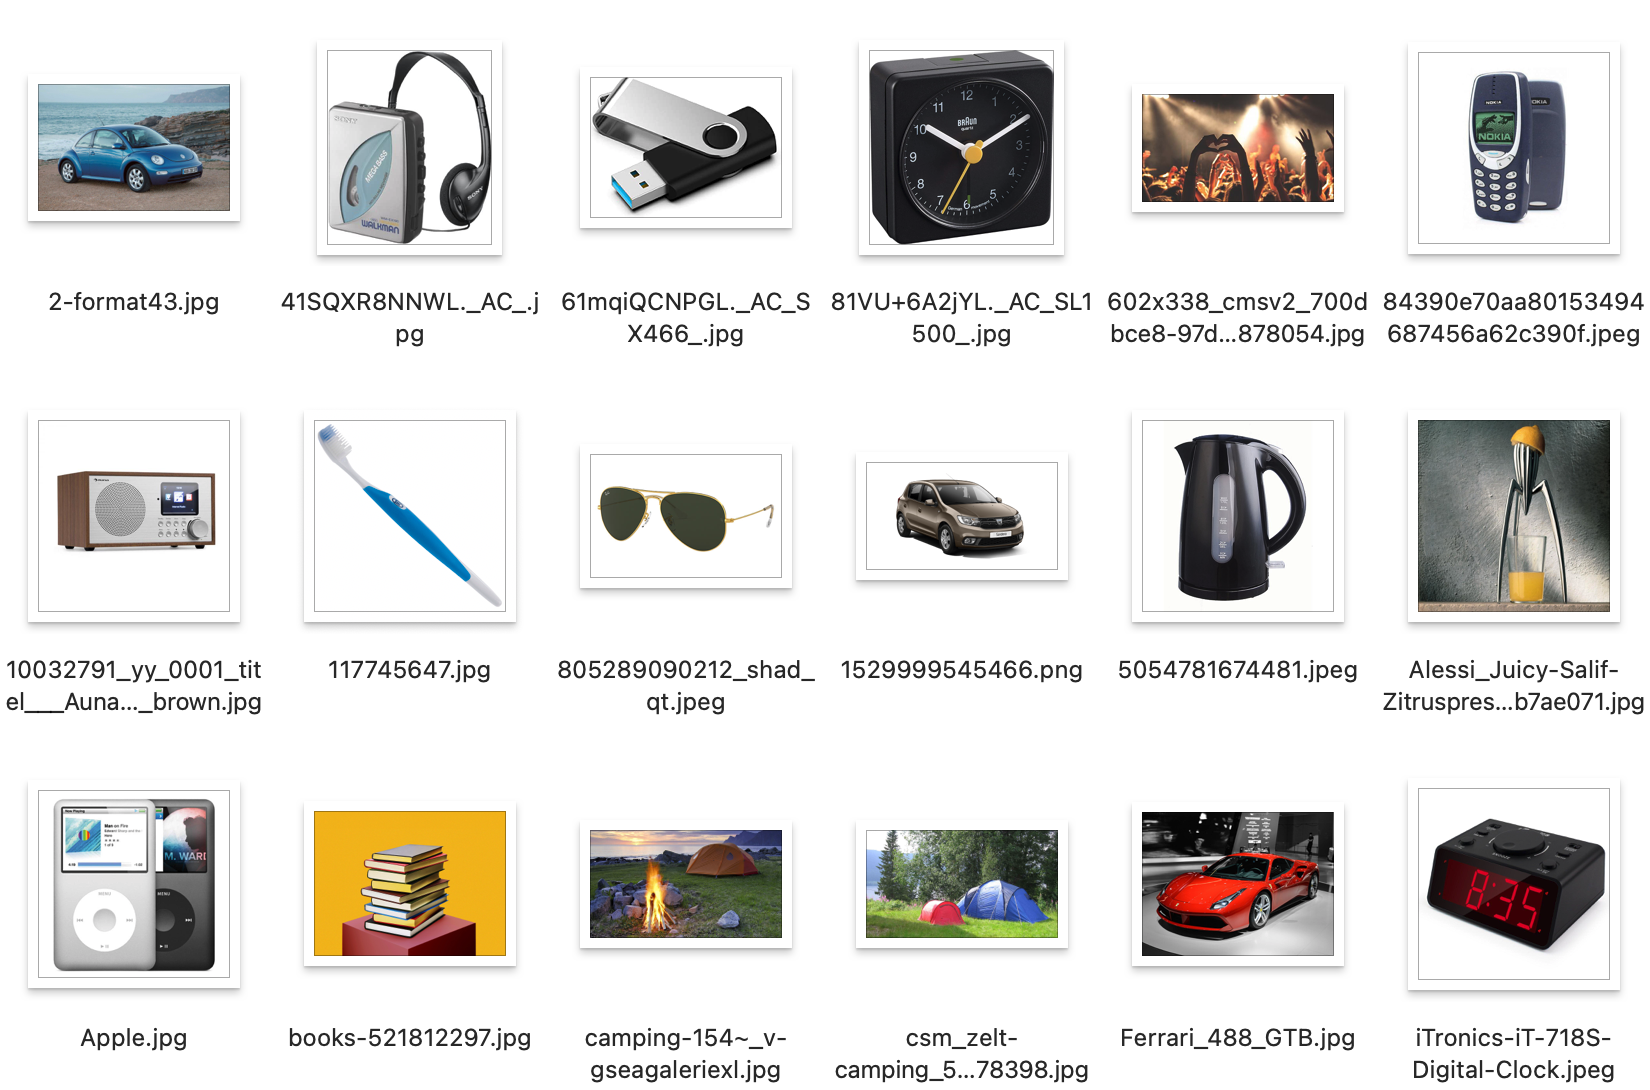
\includegraphics[width=1.19\linewidth]{fig17.png}
  \caption{Sample of images to be used in the association survey on our \href{https://meaning.pub}{website}}
  \label{fig:figure17}
\end{figure}
\vspace*{0.5em}

With the results from the word association survey in Figure \ref{tab:survey1-results} we could design a survey using terms we know people understand.

We will ask participants to rate descriptors on a Likert scale from 0 (not relevant at all) to 4 (completely relevant).
We will also include in the list of descriptors the results from the first phase of our research using NLP.
This survey will be contextualised with autonomous vehicles while the first survey was just about the terms and did not use our newly-defined context.


In future development, this survey will be sent out to the public.
From the results, we expect to find connections with our three categories of meaning.

%===================================

\subsection{Results}

The image association survey could provide us with clearer results as in products we can make a strong impression visually.
We used the findings from the previous survey to inform our image choices and enriched the options with pictures.

%\vspace*{1.2em}
%\begin{figure}[!htbp]
%  \hspace*{-3.666em}
%  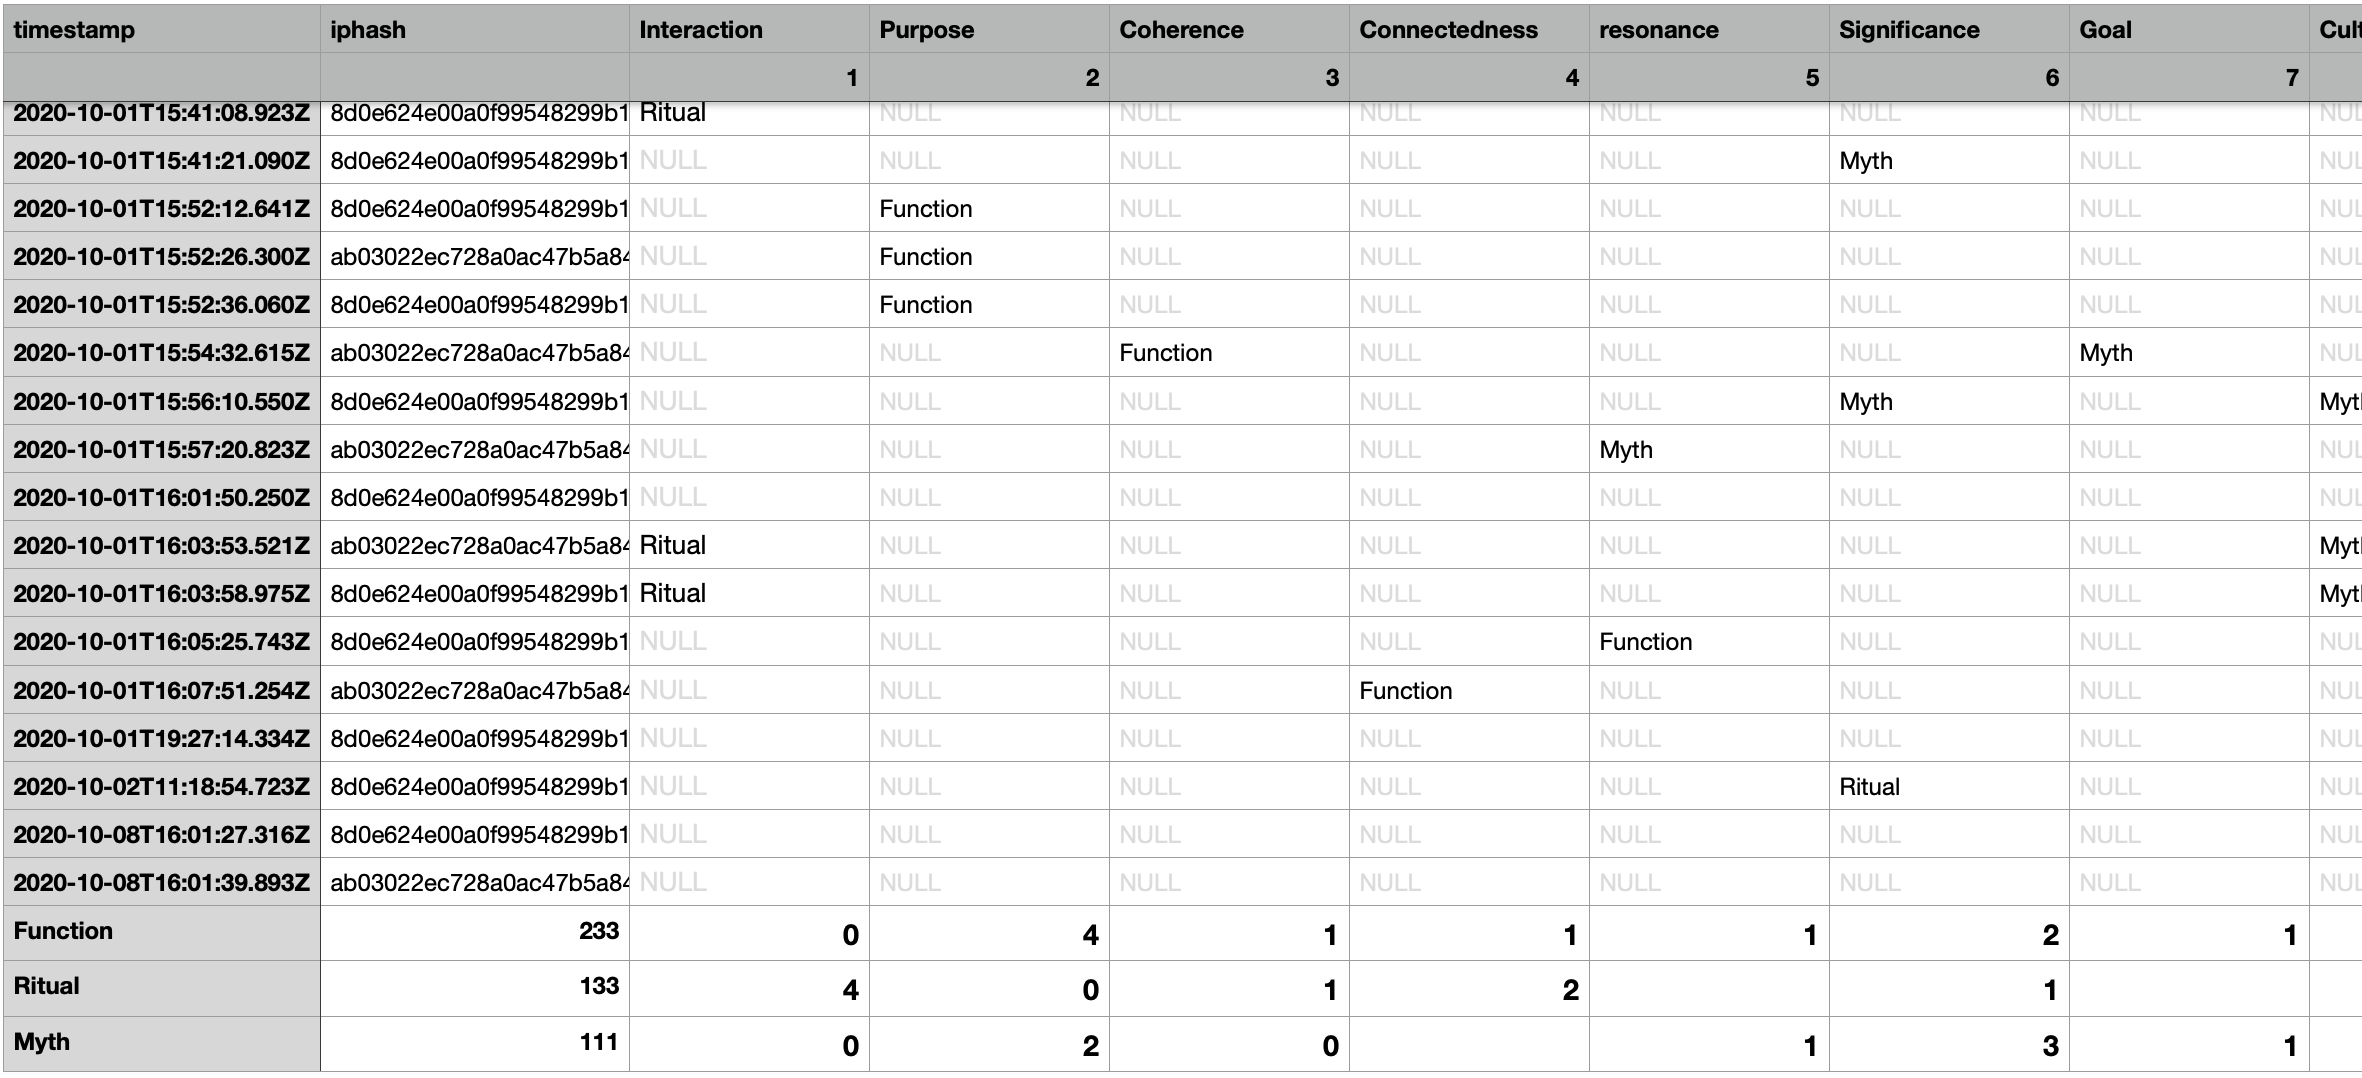
\includegraphics[width=1.19\linewidth]{fig18.png}
%  \caption{Results from the word association survey}
%  \label{fig:figure18}
%\end{figure}
%\vspace*{1.2em} 

In the word survey in Figure \ref{fig:figure16}, some terms had clear association to a given category (Reduces Risk scored 7 points in Function and none in Ritual and Myth) and other terms gave us ambivalent results (Memorability scored one point in each category).
Drawing conclusions from this, we can classify clear winners as such, but close contenders need more testing as the distribution could simply be linked to too few picks in the random word presenter.

With image association, we can also gain more data as we do not know what part of the image drew the person to make the meaning association. 
Further research is necessary and a freeform component will be required to catch the information that could have been lost in our design of the survey by excluding possibilities.

%===================================

\section{Identifying Patterns}

The image survey can help us find connections between products or product aspects with function, ritual and myth.
Our goal is to define a framework for the industry. 
As such, our decision to focus on the automotive sector with autonomous cars was the right one. 
However, as it stands we cannot make a definitive connection between our results and identifiable patterns.
We would have liked, for example, to be able to state that if a manufacturer desires the user to feel safety in using the product, the manufacturer would need to incorporate features A and B into their product while using a design language reminding people of X and Y.

As it stands, we cannot make such statements and further research is required.

%===================================

\section{Conclusion and Next Steps}

In concluding our previous chapter, we established a list of next steps. 
Some of these have been addressed in this chapter, while others have been deemed unnecessary or contrary to our direction given our newfound context.

We have not gone back to NLP since the context demands that we shift our focus to input from people.
There are no linguistic corpora that are built on AV language. 
We therefore depend on the answers from surveys and existing research papers. 
There are thousands of these papers, but we'd need hundreds of thousands for machine learning.
What we can do, is to manually review these papers.

One next step would be to define a set of criteria to be used to find more relevant research. 
For example, to look at symbolism in cars, or issues in the automotive industry.

In the coming months we plan on forming a proposal for continued research in the fields and to open up the topic to PhD candidates.

%===================================

\bibliography{d4mbib}
\bibliographystyle{ieeetr}

\end{flushleft}
\end{document}
